\documentclass[twoside,10pt]{article}

\usepackage[T1]{fontenc}
\usepackage{lmodern}
\usepackage{amsmath,amsthm,amssymb,amsfonts}
\usepackage{mathtools}
\usepackage{booktabs}
\usepackage{array}
\usepackage{float}
\usepackage{tikz}
\usepackage[letterpaper,total={5.5in,8in},vmarginratio=1:1,
  hmarginratio=1:1,headsep=21pt]{geometry}
\usepackage[small,labelfont=bf,labelsep=period]{caption}
\usepackage{xcolor}
\usepackage[breaklinks=true,linktocpage=true]{hyperref}

\numberwithin{equation}{section}

\newtheoremstyle{slbody}
  {8pt}
  {8pt}
  {\normalfont\slshape}
  {}
  {\bfseries}
  {.}
  {0.5em}
  {\thmname{#1}\thmnumber{ #2}%
   \thmnote{ {\normalfont\itshape(\ignorespaces#3\unskip)}}}
\theoremstyle{slbody}
\newtheorem{theorem}{Theorem}
\newtheorem{lemma}[theorem]{Lemma}
\newtheorem{proposition}[theorem]{Proposition}
\newtheorem{corollary}[theorem]{Corollary}
\theoremstyle{definition}
\newtheorem{definition}[theorem]{Definition}
\theoremstyle{remark}
\newtheorem*{remark}{Remark}
\numberwithin{theorem}{section}

\renewcommand{\qedsymbol}{$\blacksquare$}

\DeclareMathOperator{\Tur}{Tur}
\DeclareMathOperator{\disc}{disc}
\newcommand{\eps}{\varepsilon}
\newcommand{\coeff}[1]{[#1]\,}
\newcommand{\loglink}[1]{%
  \href{https://github.com/skypher/kraw/blob/v1.0.6/certificates/#1.txt}{\texttt{#1}}}

\newcommand{\shorttitle}{MONOTONICITY OF KRAWTCHOUK TUR\'AN DETERMINANTS}
\newcommand{\shortauthors}{LESLIE P. POLZER}
\newcommand{\paperclassification}{Primary 33C45; Secondary 05E05, 05E30, 26D05}
\newcommand{\paperkeywords}{Krawtchouk polynomials, Tur\'an determinant,
  Schur function, character value, unimodality, three-term recurrence,
  exact computation}
\newcommand{\paperaffiliation}{Independent Researcher}
\newcommand{\paperemail}{polzer@fastmail.com}
\newcommand{\paperversion}{Version 1.0.8}
\newcommand{\paperdate}{September 5, 2026}

\medmuskip=4mu
\thickmuskip=8mu
\setlength{\emergencystretch}{2em}

\hypersetup{
  colorlinks=true,
  linkcolor=purple,
  urlcolor=purple,
  citecolor=blue!80!black,
  pdftitle={Monotonicity of Tur\'an determinants for binary Krawtchouk polynomials},
  pdfauthor={Leslie P. Polzer},
  pdfkeywords={Krawtchouk polynomials, Tur\'an determinant, unimodality}
}

\makeatletter
\def\tagform@#1{%
  \maketag@@@{(\ignorespaces\oldstylenums{#1}\unskip\@@italiccorr)}}
\renewcommand{\eqref}[1]{%
  \textup{{\normalfont(\oldstylenums{\ref{#1}}}\normalfont)}}

\renewcommand{\@seccntformat}[1]{\csname the#1\endcsname.\enspace}
\renewcommand{\section}{%
  \@startsection{section}{1}{\z@}%
    {-3.5ex \@plus -1ex \@minus -.2ex}%
    {2.3ex \@plus .2ex}%
    {\normalfont\large\bfseries}}
\renewcommand{\subsection}{%
  \@startsection{subsection}{2}{\z@}%
    {-3.25ex\@plus -1ex \@minus -.2ex}%
    {1.5ex \@plus .2ex}%
    {\normalfont\normalsize\bfseries}}
\renewcommand{\subsubsection}{%
  \@startsection{subsubsection}{3}{\z@}%
    {-3.25ex\@plus -1ex \@minus -.2ex}%
    {1.5ex \@plus .2ex}%
    {\normalfont\normalsize\bfseries}}
\renewcommand{\paragraph}{%
  \@startsection{paragraph}{4}{\z@}%
    {1.5ex \@plus 1ex \@minus .2ex}%
    {-0.7em}%
    {\normalfont\normalsize\bfseries}}

\newcommand{\ps@bookheader}{%
  \renewcommand{\@oddfoot}{\hfil}%
  \renewcommand{\@evenfoot}{\hfil}%
  \renewcommand{\@oddhead}{%
    \ifnum\value{page}>1
      {\small\hfil\shortauthors}\hfil\thepage
    \else
      \hfil
    \fi}%
  \renewcommand{\@evenhead}{%
    \thepage\hfil\small\shorttitle\hfil}}
\pagestyle{bookheader}
\raggedbottom

\renewcommand{\maketitle}{%
  \begin{center}
    {\large\bfseries\@title}\\
    \vskip24pt
    \ifx\@author\@empty
      \mbox{}\par
    \else
      {\scshape\@author}\par
      \medskip
      {\small\paperaffiliation}\par
      \smallskip
      {\small\texttt{\paperemail}}\par
      \smallskip
      {\small\@date}\par
    \fi
    \vskip24pt
  \end{center}}

\renewenvironment{abstract}
  {\quotation\noindent\small{\bfseries\abstractname.\enspace}}
  {\endquotation}
\makeatother

\begin{document}

\title{Monotonicity of Tur\'an determinants\\
for binary Krawtchouk polynomials}

\author{Leslie P. Polzer}

\date{\paperversion\\\paperdate}

\maketitle

\begin{abstract}
Let $M,Q\ge0$ be integers, set $D=M+Q$, and define
$p_s=\coeff{w^s}(1+w)^M(1-w)^Q$, with $p_s=0$ outside $0\le s\le D$.
These are the binary Krawtchouk values $K_s(Q;D)$ in the generating-function
normalization.  We prove that the Tur\'an determinants
$\Tur(s)=p_s^2-p_{s-1}p_{s+1}$ satisfy
\[
  \Tur(s)\ge\Tur(s+1)
  \qquad (\lceil D/2\rceil\le s\le D).
\]
Consequently, the determinants form a symmetric weakly unimodal sequence
and satisfy $\Tur(s)\ge1$ for every $0\le s\le D$.  By the dual
Jacobi--Trudi identity, they are the rectangular Schur values
$s_{(2^s)}(1^M,(-1)^Q)$; for $D\ge1$, this gives positivity and unimodality
for a family of general linear character values at involutions.  The proof
combines recurrence comparisons in infinite regions, exact symbolic
certificates for finitely many parameter families, and an exhaustive
integer-arithmetic computation for the remaining finite cases.  Source
programs and deterministic replay logs are available in the accompanying
repository.
\vskip5pt
\noindent\textbf{Keywords.}\enspace\paperkeywords
\vskip5pt
\noindent\textbf{MSC2020 Classification.}\enspace
\paperclassification
\end{abstract}

\vskip24pt
\baselineskip=13.5pt

\section{Introduction and main theorem}\label{sec:intro}

\subsection{The theorem}\label{subsec:krawtchouk-form}

Fix integers $M,Q\ge 0$, set $D=M+Q$, and define the integer sequence
\begin{equation}\label{eq:pdef}
  p_s \;=\; \coeff{w^s}(1+w)^M(1-w)^Q, \qquad s=0,1,\dots,D,
\end{equation}
with $p_s=0$ outside $0\le s\le D$.  These are binary Krawtchouk values:
with the standard generating function
$\sum_k K_k(x;N)\,w^k=(1+w)^{N-x}(1-w)^x$ one has $p_s=K_s(Q;D)$, the
degree-$s$ binary (symmetric, $p=\tfrac12$) Krawtchouk polynomial of length
$D$ evaluated at the integer point $Q$.  Define the \emph{Tur\'an determinant} and the \emph{Tur\'an step} of this
sequence,
\begin{equation}\label{eq:Tdef}
\begin{aligned}
  \Tur(s) &\;=\; p_s^2-p_{s-1}p_{s+1},\\
  T_s &\;=\; \Tur(s)-\Tur(s+1)
    \;=\; p_s^2+p_sp_{s+2}-p_{s+1}^2-p_{s-1}p_{s+1}.
\end{aligned}
\end{equation}

\begin{theorem}[Main Theorem]\label{thm:main}
For all integers $M,Q\ge 0$ and $s$ with
$\lceil D/2\rceil\le s\le D$,
\[
  T_s \;\ge\; 0 .
\]
Equivalently, $s\mapsto\Tur(s)$ is non-increasing on the top half.  Since
$p_{D-s}=(-1)^Qp_s$, the sequence $\Tur(s)$ is symmetric about $D/2$ and
therefore weakly unimodal.
\end{theorem}

The following two corollaries are immediate by telescoping from the top end
($p_D=(-1)^Q$, $p_{D+1}=0$, so $\Tur(D)=1$).

\begin{corollary}\label{cor:positivity}
For all $M,Q\ge 0$:
\begin{enumerate}
\item $\Tur(s)\ge 1$ for every $0\le s\le D$, with sharp
  constant $1$;
\item $\Tur(s)\le\Tur(\lceil D/2\rceil)$ for $0\le s\le D$.
\end{enumerate}
\end{corollary}

\begin{corollary}[adjacent coefficient lattices]\label{cor:lattice}
For $0\le s\le D$, the two adjacent coefficient vectors
\[
 v_s=(p_{s-1},p_s),\qquad v_{s+1}=(p_s,p_{s+1})
\]
span a full-rank sublattice $L_s\subseteq\mathbb Z^2$ of index
$[\mathbb Z^2:L_s]=\Tur(s)$.  These lattice indices are symmetric and
weakly increase from either endpoint toward the center.
\end{corollary}

\begin{proof}
The determinant of the ordered column matrix is
$p_{s-1}p_{s+1}-p_s^2=-\Tur(s)$.  Hence its absolute determinant, and
therefore the lattice index, equals $\Tur(s)$ by
Corollary~\ref{cor:positivity}.  The asserted ordering is the Main Theorem and
reflection.
\end{proof}

For example, take $(M,Q)=(5,2)$.  Then
\[
 (p_s)_{s=0}^7=(1,3,1,-5,-5,1,3,1),
\qquad
 \bigl(\Tur(s)\bigr)_{s=0}^7=(1,8,16,30,30,16,8,1).
\]
The coefficients oscillate, while their Tur\'an determinants remain positive,
symmetric, and ordered toward the center.

Classical Tur\'an inequalities concern the sign of
$P_n(x)^2-P_{n-1}(x)P_{n+1}(x)$ for a fixed degree index $n$ and an argument
$x$ in the orthogonality interval \cite{szego48}.  Theorem~\ref{thm:main}
instead concerns monotonicity in the degree index (equivalently, the
generating-function coefficient index) at a fixed integer argument.  The
inequality $T_s\ge0$ can fail when the integer argument $Q$ is replaced by a
real $q$.  More precisely, for $q\in[0,D]$ define the coefficients by the
same formal generating series
\[
 [w^s](1+w)^{D-q}(1-w)^q,
\]
then at $(D,q,s)=(4,\frac87,2)$ one obtains
$T_2=-1430/117649<0$.

Closely related inequalities for binary Krawtchouk polynomials, their zeros,
and their Christoffel--Darboux kernels were studied by Krasikov and Litsyn
\cite{krasikovlitsyn96} and Krasikov
\cite{krasikov-cd,krasikov-laguerre,krasikov-turan}.
In particular, the inequality recorded in
\cite[Theorem~5, (18), p.~79]{krasikov-turan} couples adjacent Tur\'an
determinants in an exponential-coefficient normalization.
Theorem~\ref{thm:main} orders the determinants in the ordinary coefficient
normalization at a fixed integer argument.  Section~\ref{subsec:normalization}
explains the role of normalization, and Section~\ref{sec:related} gives a
detailed comparison with these results and the character literature.

\subsection{Schur-character interpretation}\label{subsec:schur}

Let
\[
 z=(\underbrace{1,\dots,1}_{M},
    \underbrace{-1,\dots,-1}_{Q}),
\]
and write $e_r(z)$ and $s_\lambda(z)$ for the elementary and Schur
symmetric functions, respectively.  As usual, $(2^s)$ denotes the
rectangular partition with $s$ rows of length $2$.

\begin{proposition}[Schur-character interpretation]\label{prop:schur}
For every $0\le s\le D$,
\begin{equation}\label{eq:schur-character}
 \Tur(s)=s_{(2^s)}(z).
\end{equation}
When $D\ge1$, this is the irreducible polynomial-character value of
$\mathrm{GL}_D(\mathbb C)$
\[
 \chi_{(2^s)}\!\left(\operatorname{diag}(I_M,-I_Q)\right).
\]
The rectangle-complement identity gives
$s_{(2^s)}(z)=s_{(2^{D-s})}(z)$ independently of the Main Theorem.
\end{proposition}

\begin{proof}
The generating function in \eqref{eq:pdef} is
$\prod_{i=1}^D(1+z_iw)$, so $p_r=e_r(z)$.  Since the conjugate of
$(2^s)$ is $(s,s)$, the dual Jacobi--Trudi identity
\cite[Chapter~I, (3.5), p.~41]{macdonald95} gives
\[
 s_{(2^s)}(z)
 =\det\begin{pmatrix}e_s(z)&e_{s+1}(z)\\
                      e_{s-1}(z)&e_s(z)
       \end{pmatrix}
 =p_s^2-p_{s-1}p_{s+1}.
\]
Schur polynomials are the irreducible polynomial characters of the general
linear group; see
\cite[Chapter~I, Appendix~A, (8.2) and (8.4), pp.~162--163]{macdonald95}.
Finally, for a
partition $\lambda$ inside the $2\times D$ rectangle, with rectangle
complement $\lambda^c$,
\[
 s_\lambda(z_1^{-1},\dots,z_D^{-1})
 =(z_1\cdots z_D)^{-2}s_{\lambda^c}(z_1,\dots,z_D).
\]
Here $z_i^{-1}=z_i$, $(z_1\cdots z_D)^2=1$, and the complement of
$(2^s)$ is $(2^{D-s})$, proving the symmetry.
\end{proof}

Thus Theorem~\ref{thm:main} and Corollary~\ref{cor:positivity} say that
the rectangular character values in \eqref{eq:schur-character} are positive
integers and form a symmetric weakly unimodal sequence as the rectangle
height $s$ varies.  For $Q>0$, the diagonal matrix has negative eigenvalues,
so ordinary Schur positivity does not by itself determine the sign.
The character interpretation identifies a
canonical representation-theoretic object and suggests seeking a
cancellation-free branching or restriction interpretation of the ordered
differences $T_s$.

\subsection{Adjacent minors and lattice indices}

For a fixed integer argument $Q$, the values $(p_s)_{s=0}^D$ form a row of
the binary Krawtchouk matrix.  The Toeplitz matrix formed from this
coefficient row has adjacent $2\times2$ minors of the form
\[
 \Tur(s)=
 \det\begin{pmatrix}p_s&p_{s+1}\\p_{s-1}&p_s\end{pmatrix}.
\]
Corollary~\ref{cor:lattice}
identifies these minors with the indices of the lattices generated by
successive coefficient vectors.  This connects the theorem with minor and
kernel inequalities in Hamming-scheme spectral analysis.  The generating
function, standard recurrences, and normalizations for Krawtchouk polynomials
may be found in \cite[Section~9.11]{koekoek-lesky-swarttouw}.

\subsection{Normalization}\label{subsec:normalization}

The normalization in \eqref{eq:pdef} is part of the statement.  If
$q_s=c_s p_s$, then
\[
 q_s^2-q_{s-1}q_{s+1}
 =c_s^2p_s^2-c_{s-1}c_{s+1}p_{s-1}p_{s+1}.
\]
Thus a Tur\'an determinant is merely rescaled by a positive factor for every
sequence $p$ only when $c_s^2=c_{s-1}c_{s+1}$, that is, when $(c_s)$ is
geometric.  Degree-dependent orthonormal or endpoint normalizations of
Krawtchouk polynomials therefore do not preserve
Theorem~\ref{thm:main}.

The coefficient normalization is natural here because it is integral at the
integer arguments under consideration, it has the exact reflection
$p_{D-s}=(-1)^Qp_s$, and it fixes the endpoint $\Tur(D)=p_D^2=1$.
The last two features turn top-half monotonicity into symmetric weak
unimodality and the sharp lower bound of Corollary~\ref{cor:positivity}.
Section~\ref{sec:related} compares this statement with Tur\'an inequalities
in other normalizations.

\subsection{Guide to the proof}\label{subsec:guide}

The top half $\{2s\ge D\}$ is divided into the bulk, flow, center, and gap
regions.  A positive-semidefinite quadratic form treats the bulk, and a
Riccati comparison treats the flow region.  The remaining gap is handled by
fixed-offset certificates, fixed-argument certificates, and two
parity-dependent recurrence arguments.  Figure~\ref{fig:coverage} and
Table~\ref{tab:coverage} summarize the decomposition; the proof is assembled
in Section~\ref{sec:assembly}.

We assume $x=M-Q\ge 0$ without loss of generality.  Indeed, $T_s$ is
invariant under $M\leftrightarrow Q$: the substitution $w\mapsto-w$ sends
$p_s$ to $(-1)^sp_s$, and every product in $T_s$ has even index sum.

\subsection{Computer-assisted components}\label{subsec:proof-status}

Three kinds of argument occur below.  First, the arguments for the bulk,
center, flow region, and gap cells with even $Q$ are given in the text;
their accompanying programs
replay algebraic identities and finite diagnostics but do not replace the
written implications.  Second, the finite-offset families, the fixed-argument
families, and one polynomial-sign lemma for gap cells with odd $Q$ are
computer-assisted results: the text states their exact inputs, domains, and
acceptance conditions, while the source programs construct and check the
finite polynomial obligations.  Third, Proposition~\ref{prop:finite-scan} is
an exhaustive computation in integer arithmetic over a declared finite set.

Every proof decision in the programs uses integer or rational arithmetic.
A second C++ implementation checks the decisive exported polynomial
witnesses and repeats the finite scan using a different coefficient
construction.  Section~\ref{sec:machine} specifies the certificate rules,
software dependencies, and theorem-by-theorem inventory.

\section{Notation and recurrence}\label{sec:reduction}

\subsection{Notation}\label{subsec:notation}

Throughout:
\begin{align*}
  &M,Q\in\mathbb Z_{\ge0};\quad D=M+Q;\quad x=M-Q\ge 0;\\
  &p_s=\coeff{w^s}(1+w)^M(1-w)^Q \text{ (integers; } p_s=0 \text{ off } [0,D]);\\
  &s \text{ top-half index, } D/2\le s\le D;\quad u=2s-D\ge 0
    \text{ (top-half offset)};\\
  &U=(u+1)^2;\quad E=(D+3)^2;\\
  &\Tur(s)=p_s^2-p_{s-1}p_{s+1};\quad T_s=\Tur(s)-\Tur(s+1);\\
  &k=D-s \text{ (distance from the top} = (D-u)/2\text{)} .
\end{align*}
Reflection: $p_{D-j}=(-1)^Qp_j$ for all $j$ (substitute $w\to 1/w$).  The
top initial values are $p_D=(-1)^Q$ and $p_{D-1}=(-1)^Qx$.  Logarithmic
differentiation of the generating function gives the step-$1$ recurrence
\begin{equation}\label{eq:recurrence}
  (s+1)\,p_{s+1} \;=\; x\,p_s + (s-1-D)\,p_{s-1} .
\end{equation}
\begin{lemma}[no consecutive zeros]\label{lem:no-consecutive-zeros}
For $0\le j\le D$, the two consecutive values $p_j,p_{j+1}$ cannot both
vanish.
\end{lemma}
\begin{proof}
If $j=0$, the assumption contradicts $p_0=1$.  If $1\le j\le D$ and
$p_j=p_{j+1}=0$, then \eqref{eq:recurrence} at index $j$ gives
$p_{j-1}=0$ because $j-1-D\ne0$.  Iteration gives $p_0=0$, again a
contradiction.
\end{proof}
We write $\eps=(-1)^Q$ and $\binom{n}{k}$ for binomial coefficients.  In the
gap sections (Sections~\ref{sec:collapse}--\ref{sec:oddmin}), we relabel
the exponents when necessary so that $0\le Q\le M$; thus $Q$ denotes the
smaller exponent.

\subsection{Finite verification}\label{subsec:scans}

A \emph{cell} is an integer triple $(M,Q,s)$ with $M,Q\ge0$ and
$\lceil(M+Q)/2\rceil\le s\le M+Q$.  We also express cells in the
coordinates $(D,x,u)$ defined above; these satisfy
$u\equiv x\equiv D\pmod2$.

\begin{proposition}[finite verification]\label{prop:finite-scan}
The inequality $T_s\ge0$ holds for every $M,Q\ge0$ with $D\le1200$ and
every $\lceil D/2\rceil\le s\le D$.
\end{proposition}

\begin{proof}
The recurrence \eqref{eq:recurrence}, initialized by $p_0=1$ and $p_1=x$,
was evaluated with GMP integers for all such triples.  The computation
examined $289{,}261{,}901$ cells and found no negative value.  Exact division
was checked before every recurrence step.  The recurrence-built values were
checked against the defining binomial convolution for every coefficient with
$D\le12$ and at deterministic indices in six larger rows, reaching
$D=1200$.  The program, output, and hash are listed in
Section~\ref{sec:machine}.
\end{proof}

A separate Python computation verifies the recurrence for $M,Q\le30$
and checks $T_s\ge0$ directly for $M,Q\le90$.

\section{Quadratic form and regime decomposition}\label{sec:regimes}

\subsection{The bulk band}

\begin{theorem}[quadratic-form identity and the bulk band]\label{thm:bulk}
Eliminating $p_{s+2}$ and $p_{s-1}$ from $T_s$ by the step-$1$ recurrence
\eqref{eq:recurrence} gives the exact identity
\begin{equation}\label{eq:qform}
\begin{gathered}
  T_s \;=\; A\,p_s^2 + B\,p_sp_{s+1} + C\,p_{s+1}^2,\\
  A=\frac{u+2}{s+2},\qquad
  B=\frac{-x(u+1)}{(D+1-s)(s+2)},\qquad
  C=\frac{u}{D+1-s},
\end{gathered}
\end{equation}
with negative discriminant
\begin{equation}\label{eq:disc}
  4AC-B^2 \;=\;
  \frac{u(u+2)\bigl((D+3)^2-(u+1)^2\bigr)-x^2(u+1)^2}
       {\bigl((D+1-s)(s+2)\bigr)^2} .
\end{equation}
Hence for $u\ge 1$, writing $U=(u+1)^2$, $E=(D+3)^2$ (note $u(u+2)=U-1$):
\begin{equation}\label{eq:bulk}
  x^2U \;\le\; (U-1)(E-U) \quad\Longrightarrow\quad T_s\ge 0
\end{equation}
  without further information about the sequence.  The condition defines the
  bulk band $U\in[U_-,U_+]$, where
  \[
    U_\pm=\frac{h\pm\sqrt{h^2-4E}}2,\qquad h:=E+1-x^2,
  \]
  are the roots of $U^2-hU+E=0$.
\end{theorem}

\begin{proof}
Substitute \eqref{eq:recurrence} for $p_{s+2}$ and $p_{s-1}$ in
\eqref{eq:Tdef}; simplification gives \eqref{eq:qform} and
\eqref{eq:disc}.  The displayed roots are real throughout the parameter
domain: since $0\le x\le D$,
\[
 h=E+1-x^2\ge (D+3)^2+1-D^2=6D+10>2(D+3)=2\sqrt E.
\]
If $u\ge1$, then $A,C>0$, and the quadratic form is positive semidefinite
whenever $4AC-B^2\ge0$.
\end{proof}

\begin{remark}[sharpness]\label{rem:sharpness}
The \emph{sign} of the negative discriminant is unchanged under the indicated
basis changes: expressing $T_s$ in a shifted recurrence basis multiplies the
negative discriminant by a positive square.  For example, the negative
discriminant in the $(p_{s-2},p_{s-1})$ basis is the displayed one times
\[
 \left(\frac{(D+1-s)(D+2-s)}{s(s+1)}\right)^2.
\]
Thus no change among the shifted recurrence bases makes the form
positive semidefinite outside the bulk band.  The remaining arguments
therefore use additional information from the Krawtchouk recurrence.
\end{remark}

\subsection{The center}

\begin{theorem}[central identity, $u=0$, $D$ even]\label{thm:center}
By reflection ($p_{D-j}=(-1)^Qp_j$): for $Q$ odd, $p_{D/2}=0$ and
$T_{D/2}=0$ identically.  For $Q$ even, the reflection constraint
$p_{s-1}=p_{s+1}$ at $s=D/2$ collapses the recurrence to the rank-one
relation $(D+2)\,p_{s+1}=x\,p_s$, and
\begin{equation}\label{eq:center}
  T_{D/2} \;=\; \frac{4\,p_{D/2}^2\,\bigl((D+2)^2-x^2\bigr)}
                     {(D+2)^2(D+4)} \;\ge\; 0,
\end{equation}
with equality if and only if $p_{D/2}=0$.
\end{theorem}

\begin{proof}
If $Q$ is odd, reflection gives $p_{D/2}=0$ and
$p_{D/2-1}=-p_{D/2+1}$, which makes the four terms in $T_{D/2}$ cancel.
If $Q$ is even, reflection gives $p_{s-1}=p_{s+1}$ at $s=D/2$.
Substitution in \eqref{eq:recurrence} yields
$(D+2)p_{s+1}=xp_s$; inserting this relation into \eqref{eq:Tdef} and using
the recurrence once more for $p_{s+2}$ gives \eqref{eq:center}.  Its remaining
factor is strictly positive because
\[
 (D+2)^2-x^2\ge (D+2)^2-D^2=4D+4>0.\qedhere
\]
\end{proof}

The recurrence arguments in Sections~\ref{sec:evenflow} and~\ref{sec:oddmin}
start from reflection constraints at the center.

When $M$ and $Q$ are both odd, $D$ is even and
$T_{D/2}=0$.  This completely describes equality at the central step.  If
$D$ is even, then $M,Q$ have the same parity.  The odd--odd case is the
first case of Theorem~\ref{thm:center}; in the even--even case,
$p_{D/2}=0$ together with
$(D+2)p_{D/2+1}=xp_{D/2}$ would give two consecutive zeros, contrary to
Lemma~\ref{lem:no-consecutive-zeros}.  We do not claim a classification of
equality at noncentral steps.

\subsection{The flow region: Riccati comparison}

\begin{theorem}[flow region]\label{thm:flow}
Let $k=D-s\ge 1$.  Whenever its radicand is nonnegative, let
\[
 w_s=\sqrt{x^2-4k(D+1-k)}
\]
denote the nonnegative square root.  On the flow region $w_s^2\ge 0$,
equivalently
$(u+1)^2\ge(D+1)^2-x^2$ by the identity
$(D+1)^2-(u+1)^2=4(s+1)(D-s)$, one has $T_s\ge 0$.
\end{theorem}

\begin{proof}
The flow region with $k\ge1$ is empty when $x=0$, so assume $x>0$.
On the top half, $0\le k\le D/2$, and
$k\mapsto4k(D+1-k)$ is increasing.  Hence if the target index is in the
flow region, so is every index between it and $D-1$; the following downward
induction runs on this connected tail.  The center $u=0$ cannot lie in the
flow region, because there $4k(D+1-k)=D(D+2)>D^2\ge x^2$.  Thus $u\ge1$
and the quadratic-form coefficient $C$ is positive throughout the tail.

Use the ratio variable $r_s=p_{s+1}/p_s$.  The top initial values
$p_D=(-1)^Q$, $p_{D-1}=(-1)^Qx$ give $r_{D-1}=1/x$, and the recurrence
gives the downward M\"obius flow
\[
  r_{s-1} \;=\; \frac{D+1-s}{\,x-(s+1)\,r_s\,} .
\]
Set $\phi_s=(x+w_s)/2$ and define the auxiliary downward Riccati flow
$y_{s-1}=x-(s+1)(D-s)/y_s$, $y_{D-1}=x$.  Then:
\begin{enumerate}
\item \emph{(comparison)}  The inequality
  $\phi_{s-1}\le x-(s+1)(D-s)/\phi_s$ reduces, after clearing denominators
  by $4(s+1)(D-s)=x^2-w_s^2$, to
  $(w_s-w_{s-1})(x+w_s)\ge 0$.  This holds because
  $w_s^2-w_{s-1}^2=4u>0$.  Induction from
  $y_{D-1}=x\ge\phi_{D-1}$ gives $y_s\ge\phi_s>0$ on the connected tail.

  Starting from $r_{D-1}=1/x=(D-(D-1))/y_{D-1}$, a simultaneous induction
  in the two displayed recurrences gives
  $r_s=(D-s)/y_s=k/y_s$.  Consequently
  $0<r_s\le k/\phi_s$, every M\"obius denominator is positive, and no
  $p_s$ in the tail vanishes.
\item \emph{(window value)}  The quadratic-form value of
  Theorem~\ref{thm:bulk} at $r=k/\phi_s$ is
  $I_1/\bigl((s+2)(D+1-s)\phi_s^2\bigr)$
  with
  \begin{equation}\label{eq:I1}
  \begin{gathered}
    I_1 \;=\; (u+2)(k+1)\,\phi_s^2 - x(u+1)\,k\,\phi_s
        + u(D-k+2)\,k^2
        \;=\; P_1+Q_1w_s,\\
    Q_1 \;=\; \tfrac12\,x(D-k+2) \;\ge\; 0,\\
    P_1 \;=\; \tfrac12\bigl[x^2(D+2-k)-2k(D^2-2Dk+3D+2k^2-2k+2)\bigr],
  \end{gathered}
  \end{equation}
  The coefficient $D+2-k$ of $x^2$ is positive.  Thus $P_1$ is increasing
  in $x^2$, and at the flow boundary $x^2=4k(D+1-k)$ it equals
  $k(D+2)(u+1)>0$.  Since also $Q_1,w_s\ge0$, this proves $I_1\ge0$
  throughout the flow region.
\item \emph{(window vertex)}  Since $C>0$, the inequality
  $k/\phi_s\le -B/(2C)$ reduces to
  \begin{equation}\label{eq:I2}
    I_2 \;=\; x(u+1)\,\phi_s - 2u(D-k+2)\,k
      \;=\; P_2+Q_2w_s ,
  \end{equation}
  where
  \[
    Q_2=\frac{x(u+1)}2,\qquad
    P_2=\frac{x^2(u+1)
      -4k(D^2-3Dk+2D+2k^2-4k)}2 .
  \]
  Since $u+1>0$, $P_2$ is increasing in $x^2$; at the flow boundary it
  equals $2k(k+1)>0$.  Hence $I_2\ge0$.
\item Since $A,C\ge 0\ge B$, the quadratic $A+Br+Cr^2$ is decreasing on
  $[0,-B/(2C)]$; by (1)--(3),
  $T_s/p_s^2=A+Br_s+Cr_s^2
  \ge(\text{value at }k/\phi_s)\ge 0$. \qedhere
\end{enumerate}
\end{proof}

\subsection{Coverage and the gap}

\begin{corollary}[coverage]\label{cor:coverage}
For $D=0$ the only cell is $s=0$ and $T_0=1$.  For $D\ge1$, every
top-half cell is covered by the top, center, bulk, or flow arguments except
the set
\begin{equation}\label{eq:gap}
  \mathcal G=\bigl\{u\ge1:x^2U>(U-1)(E-U),\quad
  U<(D+1)^2-x^2\bigr\},
\end{equation}
equivalently $\{u\ge1:U<U_-\}$.
\end{corollary}

\begin{proof}
At the flow boundary $U_0=(D+1)^2-x^2$ the bulk margin is
\[
  (U_0-1)(4D+8)-x^2 \;=\; (D^2+2D-x^2)(4D+8)-x^2 \;>\; 0
\]
for $0\le x\le D$ (decreasing linearly with $x^2$, with value $7D^2+16D$ at
$x^2=D^2$).  Hence $U_-\le U_0\le U_+$, and every top-half cell is covered
by $\{s=D\}$ ($T_D=1$), $\{u=0\}$ (Theorem~\ref{thm:center}), the bulk
($U_-\le U\le U_0$), and the flow ($U\ge U_0$), except for
\eqref{eq:gap}.
\end{proof}

\begin{lemma}[heredity of the gap]\label{lem:gap-heredity}
If $(D,x,u)$ is a gap cell and $u'\equiv u\pmod2$ satisfies
$1\le u'\le u$, then $(D,x,u')$ is also a gap cell.
\end{lemma}

\begin{proof}
Corollary~\ref{cor:coverage} identifies the gap exactly with
$1\le (u+1)^2<U_-$.  Since $(u'+1)^2\le(u+1)^2$, the same inequality holds
for $u'$.  The parity condition makes $s'=(D+u')/2$ an integer index.
\end{proof}

Using $E-x^2=(2Q+3)(2M+3)$, failure of the bulk inequality is equivalent to
\begin{equation}\label{eq:gap-lopsided}
  (2Q+3)(2M+3) \;<\; U+\frac EU-1 .
\end{equation}
Together with the non-flow condition in \eqref{eq:gap}, this characterizes
the gap.  Thus gap cells occur only when the two exponents are unequal.  An exact
census shows that the first gap cell with $u\ge4$ and $Q\ge3$ appears at $D=442$,
$(Q,u)=(3,4)$.  Over all $Q$ the first such cell is instead
$(D,Q,u)=(142,0,4)$; it is covered by Proposition~\ref{prop:qle2} before
this residual region is considered.

The \texttt{regime-decomposition} program also checks this
partition for every top-half cell with $D\le90$.

\begin{lemma}[gap strip]\label{lem:gap-strip}
After relabeling so that $Q\le M$, every gap cell satisfies
\begin{equation}\label{eq:gap-strip}
  (u+1)^2=U<U_-\le
  \frac76\,\frac{D+3}{2Q+3}.
\end{equation}
\end{lemma}

\begin{proof}
Here
\[
 h=E+1-x^2=(2Q+3)(2M+3)+1,
\]
and $h-3(D+3)=4MQ+3M+3Q+1>0$.  Thus $h>3\sqrt E$.
Since
\[
 U_-=\frac{2E}{h+\sqrt{h^2-4E}},
\]
putting $t=h/\sqrt E$ shows that
\[
 \frac{U_-}{E/h}=\frac{2t}{t+\sqrt{t^2-4}}.
\]
The last function is decreasing for $t\ge2$, and its value at $t=3$ is
$6/(3+\sqrt5)\le7/6$.  Hence $U_-\le(7/6)E/h$.
Finally $h\ge(2Q+3)(D+3)$ because $2M+3\ge D+3$ when $Q\le M$.
\end{proof}

\begin{figure}[H]
\centering
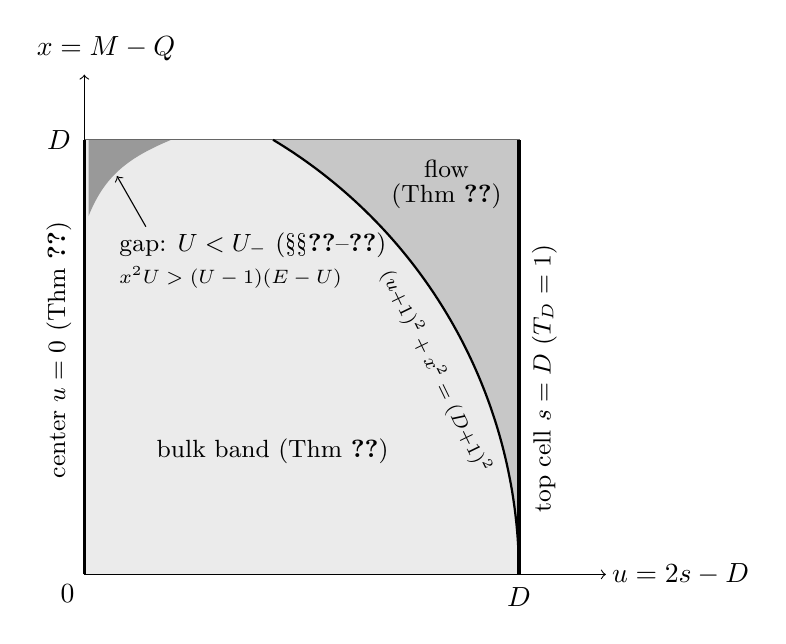
\begin{tikzpicture}[scale=0.92]
  % flow boundary: the circle (u+1)^2 + x^2 = (D+1)^2, center (-1,0),
  % radius D+1; drawn for the schematic's finite D (= 6 units), so the
  % arc runs from (D,0) to (sqrt(2D+1)-1, D).
  % bulk region: inside the arc
  \fill[black!8] (0,0) -- (6,0) arc[start angle=0, end angle=59, radius=7]
    -- (0,6) -- cycle;
  % flow region: between the arc and the top/right edges
  \fill[black!22] (6,0) arc[start angle=0, end angle=59, radius=7]
    -- (6,6) -- cycle;
  % gap wedge (qualitative), top-left, strictly inside the bulk
  \fill[black!40] (0.06,6) -- (1.2,6)
    .. controls (0.6,5.75) and (0.28,5.5) .. (0.06,4.95) -- cycle;
  % domain frame
  \draw[black!60] (0,0) rectangle (6,6);
  % flow boundary arc
  \draw[thick] (6,0) arc[start angle=0, end angle=59, radius=7];
  % center column and top cell
  \draw[very thick] (0,0) -- (0,6);
  \draw[very thick] (6,0) -- (6,6);
  % axes
  \draw[->] (0,0) -- (7.2,0);
  \node[right] at (7.15,0) {$u=2s-D$};
  \draw[->] (0,0) -- (0,6.9);
  \node[above] at (0.3,6.95) {$x=M-Q$};
  \node[below] at (6,-0.05) {$D$};
  \node[left] at (-0.05,6) {$D$};
  \node[below left] at (0,0) {$0$};
  % region labels
  \node at (2.6,1.7) {\small bulk band (Thm~\ref{thm:bulk})};
  \node at (5.0,5.6) {\small flow};
  \node at (5.0,5.22) {\small (Thm~\ref{thm:flow})};
  \node[rotate=90] at (-0.35,3.1) {\small center $u=0$ (Thm~\ref{thm:center})};
  \node[rotate=90] at (6.35,2.7) {\small top cell $s=D$ ($T_D=1$)};
  \node[rotate=-64] at (4.85,2.8) {\scriptsize $(u{+}1)^2+x^2=(D{+}1)^2$};
  % gap label with pointer, in the bulk interior below the wedge
  \draw[->] (0.85,4.8) -- (0.45,5.5);
  \node[right] at (0.35,4.55) {\small gap: $U<U_-$
    (\S\S\ref{sec:collapse}--\ref{sec:oddmin})};
  \node[right] at (0.35,4.1) {\scriptsize $x^2U>(U-1)(E-U)$};
\end{tikzpicture}
\caption{Coverage of the top half $\{2s\ge D\}$ in the $(u,x)$-plane for
fixed $D$ (schematic; lattice cells satisfy $u\equiv x\equiv D\pmod 2$).
For this schematic, the overlap of the bulk and flow regions is assigned
to the flow region, beyond the displayed circle.  The
dark gap is removed from the light bulk shading: it is the part of the
non-flow region where the bulk quadratic form is indefinite,
$\{u\ge1:U<U_-\}$.  It is treated in
Sections~\ref{sec:collapse}--\ref{sec:oddmin}.}
\label{fig:coverage}
\end{figure}

\subsection{Coverage and thresholds}
\label{subsec:coverage}

Table~\ref{tab:coverage} records which statement covers each region.
Theorems~\ref{thm:bulk}, \ref{thm:center}, \ref{thm:flow}, and
\ref{thm:offsets}, together with
Propositions~\ref{prop:collapse} and~\ref{prop:qle2}, cover every cell with
$D\le4586$; the first cell not covered by those results is
$(D,Q,u)=(4587,3,15)$.  Corollary~\ref{cor:finite-coverage} extends the
threshold to $D\le14826$, and Theorems~\ref{thm:evenflow}
and~\ref{thm:oddmin} cover all remaining cells.

The numerical cutoffs are bookkeeping constants, not conjecturally sharp
features of the inequality.  The exact scan through $D=1200$ absorbs the
finite-offset nondegeneracy remainder $D<1191$; the fixed-argument edge-flow
onsets are smaller still (at most $93$).  In the final residual region,
$x\le D-26$ is simply $x=D-2Q$ with $Q\ge13$.

\begin{table}[H]
\centering
\small
\begin{tabular}{@{}ll@{}}
\toprule
Region or slice of the gap & Covered by \\
\midrule
top cell $s=D$ & endpoint identity $T_D=1$ \\
center column $u=0$ & Theorem~\ref{thm:center} \\
bulk band $x^2U\le(U-1)(E-U)$ & Theorem~\ref{thm:bulk} \\
flow region $U\ge(D+1)^2-x^2$ & Theorem~\ref{thm:flow} \\
coverage: everything else $=$ gap & Corollary~\ref{cor:coverage} \\
gap, $u\le 3$ & Proposition~\ref{prop:collapse} \\
gap, $Q\ge3$, $4\le u\le 14$ & Theorem~\ref{thm:offsets} \\
gap, $Q\le 2$ & Proposition~\ref{prop:qle2} \\
gap, $3\le Q\le 12$ & Theorem~\ref{thm:strips} \\
gap, $u\ge 15$, $Q\ge 13$, $Q$ even & Theorem~\ref{thm:evenflow} \\
gap, $u\ge 15$, $Q\ge 13$, $Q$ odd & Theorem~\ref{thm:oddmin} \\
all cells with $D\le 1200$ & Proposition~\ref{prop:finite-scan} \\
\bottomrule
\end{tabular}
\medskip
\caption{Coverage of the proof.  Throughout the table, $Q\le M$.}
\label{tab:coverage}
\end{table}

\section{Reflection collapse and finite families}\label{sec:collapse}

The gap is next treated through two finite collections of parameter families:
fixed-offset families (Proposition~\ref{prop:collapse} and
Theorem~\ref{thm:offsets}) and fixed-argument strips
(Proposition~\ref{prop:qle2} and Theorem~\ref{thm:strips}).

\subsection{Reflection collapse: gap offsets \texorpdfstring{$u\le 3$}{u <= 3}}

\begin{proposition}[reflection collapse]\label{prop:collapse}
Every gap cell with $u\le3$ has $T_s\ge0$.
\end{proposition}

\begin{proof}
For $s=(D+u)/2$ reflection gives $p_{s-u}=(-1)^Qp_s$.  Combining this
reflection constraint with the $(u+2)$-step recurrence chain determines the ratio
$p_{s-u+1}/p_{s-u}$ as an explicit rational function of $(M,Q)$ and yields
closed forms
\[
  T_s \;=\; R_u(M,Q)\;p_{s-u}^2 .
\]
For $u=1,2,3$, with $\eps=(-1)^Q$ indicated by the superscript, the
recurrence gives
\begin{gather*}
  R_1^+ = \frac{32\,(M+2)(Q+1)}{(D+3)^2(D+5)}, \qquad
  R_1^- = \frac{32\,(M+1)(Q+2)}{(D+3)^2(D+5)}, \\[4pt]
  R_2^+ = \frac{16\,(M+1)(Q+1)\bigl[(M-Q)^2+2M^2+2Q^2+6M+6Q\bigr]}
               {x^2(D+4)^2(D+6)}, \\[4pt]
  R_2^- = \frac{32\,(M+2)(Q+2)}{(D+4)^2(D+6)}, \\[4pt]
  R_3^+ = \frac{64\,(M+2)(Q+1)\bigl[(M-Q)^2+4Q^2+12Q-1\bigr]}
               {(M-3Q-1)^2(D+5)^2(D+7)}, \\[4pt]
  R_3^- = \frac{64\,(M+1)(Q+2)\bigl[(M-Q)^2+4M^2+12M-1\bigr]}
               {(3M-Q+1)^2(D+5)^2(D+7)}.
\end{gather*}
These expressions are nonnegative in the stated range: the two terms
containing $-1$ are nonnegative for $Q\ge1$ and $M\ge1$, respectively,
while for $R_3^+$ with $Q=0$ one has $D=M\ge u=3$ (a coefficient cell
requires $u\le D$), so $M^2-1>0$.  The only potentially negative residual
values have $D<u$ and are not coefficient cells.
The collapse denominators do not vanish on the gap: $x=0$ fails the gap
inequality outright; $M=3Q+1$ gives
$16x^2-15(E-16)=-(176Q^2+416Q-16)<0$ for $Q\ge 1$; and $3M-Q+1>0$ for
$M\ge Q$.  Moreover, the seed $p_{s-u}$ cannot vanish: once the displayed
collapse denominator is nonzero, the reflection constraint and the
recurrence force $p_{s-u+1}=0$ as well, contradicting
Lemma~\ref{lem:no-consecutive-zeros}.  Thus the ratio elimination used above
is legitimate, and every gap cell with $u\le 3$ has $T_s\ge 0$.
\end{proof}

\subsection{Fraction-free constrained forms: gap offsets \texorpdfstring{$4\le u\le 14$}{4 <= u <= 14}}

\begin{theorem}[finite gap offsets]
\label{thm:offsets}
Every gap cell with $Q\ge3$ and $4\le u\le14$ has $T_s\ge0$.
\end{theorem}

\begin{proof}
For each $u$ and parity class $\eps=(-1)^Q$, the reflection constraint is
encoded fraction-free: with the scaled chain $P_i=c_i\,p_{k_0+i}$
($k_0=s-u=D-s$; $c_0=c_1=1$ and
$c_{i+1}=c_i\,(k_0+i+1)$ for $i\ge1$), the recurrence becomes
\[
 P_{i+1}=xP_i+(k_0+i-1-D)\frac{c_i}{c_{i-1}}P_{i-1}.
\]
Thus every $P_i$ has polynomial coefficients in the two seeds
$(a,b)=(p_{k_0},p_{k_0+1})$.  All scale factors used below are positive:
$k_0\ge0$ and every new factor $k_0+i+1$ is positive.  In particular,
\[
 \widetilde T:=T_s\,c_{u+1}c_{u+2}
   =\mathcal A a^2+\mathcal B ab+\mathcal C b^2
\]
is a polynomial quadratic form.  The constraint $p_s=\eps\,p_{k_0}$ reads
$\lambda a+\mu b=0$ with polynomial $\lambda,\mu$, and pure algebra gives
the two identities
\begin{equation}\label{eq:fractionfree}
  \widetilde T\,\mu^2 \;=\; G\,a^2, \qquad
  \widetilde T\,\lambda^2 \;=\; G\,b^2, \qquad
  G \;:=\; \mathcal A\mu^2-\mathcal B\lambda\mu+\mathcal C\lambda^2,
\end{equation}
at every cell satisfying the constraint, without division.  Hence $T_s\ge0$
follows at a cell whenever $G\ge 0$ there and $(\lambda,\mu)\ne(0,0)$.  The
\texttt{finite-gap-offsets} replay proves the following finite
computer-assisted certificate for each $(u,\eps)$:
\begin{enumerate}
\item \emph{(sector)}  $\mathrm{gap}(u)$ with $Q\ge 3$ forces
  $Q<M/(u+1)^2$, by the estimate
  $2Q+3<(D+3)/U+U/(D+3)$ with $(D+3)/U>8$.
  Indeed, $U<U_-\le D+3$ makes $\tau=(D+3)/U>1$, and then
  $\tau+1/\tau>2Q+3\ge9$ forces $\tau>(9+\sqrt{77})/2>8$.
  The exact census already quoted in Section~\ref{sec:regimes} (and repeated by
  this verifier) shows that no gap cell with $u\ge4$ and $Q\ge3$ has
  $D<442$, so $Q<M/25$ gives
  $M>\tfrac{25}{26}D\ge\tfrac{25}{26}\cdot442=425$.
  Since $M$ is integral, this gives $M\ge426$; all subsequent bounds require
  only $M\ge425$.
\item \emph{(two reduced constraints)}  We call a chosen reflection
  constraint a \emph{pinning}.  For the primary pinning
  $p_s=\eps p_{k_0}$, let $g_1=\gcd(\lambda_1,\mu_1)$ and factor out the
  greatest common divisor by writing
  $(\lambda_1,\mu_1)=g_1(\lambda'_1,\mu'_1)$, so
  $G_1=g_1^2G'_1$.  The same construction for the alternate pinning
  $p_{s+1}=\eps p_{k_0-1}$ gives
  $(\lambda_2,\mu_2)$, $g_2$, and $G'_2$.  The two fraction-free
  identities \eqref{eq:fractionfree} hold for each reduced constraint
  wherever its $g_r$ is nonzero.
\item \emph{(positivity)}  $G'\ge 0$ on the sector via factorization:
  even-multiplicity factors are nonnegative; odd-multiplicity factors are
  positive because their leading homogeneous form $L(t)$ is positive on
  $[0,1/(u+1)^2]$ (an exact $512$-point partition and a derivative bound),
  while explicit weighted bounds control all lower-degree terms.
  This is done for both $G'_1$ and $G'_2$.  The resulting thresholds satisfy
  $M_0(u)\le153$ through $u=14$, so the sector bound $M\ge425$
  automatically lies beyond every positivity threshold.
\item \emph{(nondegeneracy)}  For \emph{each} of the two pinnings, the
  reduced pair $(\lambda'_r,\mu'_r)$ has no common integer zero on
  the part of the sector with $M>1145$ (resultant in $Q$, integer-root
  candidates, exact check).  The omitted range is already covered by
  Proposition~\ref{prop:finite-scan}: since $Q<M/(u+1)^2\le M/25$,
  $M\le1145$ implies $D=M+Q<1191<1200$.

  Where the first common factor $g_1$ vanishes, we use the alternative
  reflection constraint $p_{s+1}=\eps\,p_{k_0-1}$.  A further resultant
  check proves that $\{g_1=0\}\cap\{g_2=0\}$ contains no integer sector
  point with $M>1145$.  Thus the second common factor is nonzero there,
  and the second reduced identities are valid.  The second reduced pair
  is nonzero by its own nondegeneracy check above.  Both $g_2\ne0$ and
  $(\lambda'_2,\mu'_2)\ne(0,0)$ are used at this cell.
\end{enumerate}
Here $G'$ in item (3) denotes either reduced form $G'_r$.  Consequently at
least one reduced identity is valid at every cell, its right-hand side is
nonnegative, and a nonzero reduced constraint coefficient forces
$\widetilde T\ge0$.  Positivity of the scale factors then gives $T_s\ge0$.
The recursive inputs, generic sign lemmas, factor degrees, domination
thresholds, and resultant-candidate reporting are stated explicitly in
Section~\ref{subsec:certificate-spec}.
\end{proof}

\paragraph{A worked finite-offset certificate.}
We illustrate the certificate construction with $u=4$ and $\eps=+1$.
After removing the common factor
$g=M-Q=x$ from $(\lambda,\mu)$, the program obtains
\[
\begin{aligned}
 \lambda'&=-\frac{x(D+4)}2,\\
 \mu'&=\frac{M^2-6MQ-2M+Q^2-2Q}{2},\\
 G'&=\frac{(M+1)(Q+1)D^2(D+2)^2(D+4)^2}{128}\,F(M,Q),
\end{aligned}
\]
where
\[
\begin{split}
F(M,Q)={}&5M^4-20M^3Q+78M^2Q^2-20MQ^3+5Q^4\\
 &+144M^2Q+144MQ^2-20M^2+472MQ-20Q^2 .
\end{split}
\]
On the certified sector put $t=Q/M<1/25$.  Dropping positive terms gives
\[
 \frac{F(M,Q)}{M^4}
 \ge \frac{13121}{3125}-\frac{20(1+t^2)}{M^2}>0
 \qquad(M\ge425).
\]
Moreover $x\ne0$ on a gap cell, so $g\ne0$ and
$\lambda'\ne0$; the alternate pinning and the resultant checks are
therefore not needed for this family's argument (the verifier still
performs them).
The identities \eqref{eq:fractionfree} therefore prove the $u=4$,
$\eps=+1$ family directly.  The other $21$ offset--parity families follow
the same construction, with the longer factor and nondegeneracy data
recorded by the certificate generator.

Together with the preceding results and Proposition~\ref{prop:qle2}, this
covers every offset $u\le14$ and every cell with $D\le4586$.

\subsection{Small-argument closed forms: \texorpdfstring{$\min(M,Q)\le 2$}{min(M,Q) <= 2}}

\begin{proposition}[$\min(M,Q)\le 2$, all $D$]\label{prop:qle2}
If $\min(M,Q)\le2$, then $T_s\ge0$ at every top-half index.
\end{proposition}

\begin{proof}
Put $v:=D-u=2(D-s)$.  For fixed $Q$, exact cancellation gives
\[
 \frac{T_s}{\binom Ms^2}=\frac{N_Q(D,u)}{\Delta_Q(D,u)}
 \qquad (u\le D-10),
\]
where $\Delta_Q>0$: after factorization it is a positive constant times
squares, positive factors $D+u+c$, and the positive factor $D+2-u$.
(Equivalently, the denominator before this sign adjustment has the single negative
factor $u-D-2$.)  The edge $v<10$ is covered by the trivial top cell when
$s=D$, and by Theorem~\ref{thm:flow} for $D\ge24$ when $s<D$.
The oriented numerators $N_Q$ are:
\begin{equation}\label{eq:S2}
\begin{aligned}
  N_0&=(D+1)(D+2)(1+u),\\
  N_1&=D(D+1)\,u(u+1)(u+2),\\
  N_2&=D(D-1)\,S_2,\\
  S_2&=c_0+c_1u+c_2u^2+c_3u^3+c_4u^4+c_5u^5\\
     &=3D(D+2)+(D+2)(3D-4)\,u-2(3D+4)\,u^2\\
     &\qquad{}-2(D-2)\,u^3+5u^4+u^5 .
\end{aligned}
\end{equation}
The $Q=0$ numerator is positive; the $Q=1$ numerator is nonnegative and
vanishes exactly at $u=0$
(Theorem~\ref{thm:center}, odd parity); and
$S_2\ge 0$ on the strip $u^2\le D/13$ by \emph{paired domination}:
\[
  13c_0+Dc_2 \;=\; D(33D+70) \;\ge\; 0, \qquad
  13c_1+Dc_3 \;=\; 37D^2+30D-104 \;\ge\; 0,
\]
with $c_4,c_5\ge 0$ (the second paired polynomial is positive for
$D\ge2$, the only relevant $Q=2$ range).

It remains to justify that this strip contains the whole $Q=2$ gap.  Here
$x=D-4$, $E=(D+3)^2$, and
$h=E+1-x^2=14D-6$.  Since $h\ge2\sqrt E$ for $D\ge3$,
rationalizing the smaller root gives
\[
 U<U_-=\frac{2E}{h+\sqrt{h^2-4E}}
 \le\frac{E}{h-\sqrt E}
 \le\frac{(D+3)^2}{13D-9}.
\]
Moreover
\[
 13(D+3)^2\le(D+13)(13D-9)
 \quad\Longleftrightarrow\quad 82D-234\ge0.
\]
Consequently $(u+1)^2\le D/13+1$, and thus
$u^2=(u+1)^2-2u-1\le D/13$ for $u\ge0$.  Off the strip
Corollary~\ref{cor:coverage} applies.  The edge cells with $D<24$ lie in
Proposition~\ref{prop:finite-scan}.
\end{proof}

\subsection{Fixed-argument strips: \texorpdfstring{$3\le Q\le 12$}{3 <= Q <= 12}}

\begin{lemma}[fixed-argument certificate]\label{lem:fixed-q-certificate}
Fix $3\le Q\le12$ and set
\[
 R_j(M,s):=\sum_{b=0}^Q(-1)^b\binom Qb
 \begin{cases}
 \displaystyle\prod_{i=0}^{j-b-1}\frac{M-s-i}{s+i+1},&j-b\ge0,\\[6pt]
 \displaystyle\prod_{i=0}^{b-j-1}\frac{s-i}{M-s+i+1},&j-b<0.
 \end{cases}
\]
On the strip $0\le u\le D-2Q-6$,
\[
 \frac{T_s}{\binom Ms^2}=R_0^2+R_0R_2-R_1^2-R_{-1}R_1.
\]
After substituting $M=D-Q$, $s=(D+u)/2$, orienting the denominator, and
removing positive content, write its numerator as
$S_Q=\sum_jc_j(D)u^j$.  On $0\le u\le D-2Q-6$ the oriented denominator is
positive.  Every negative term $c_ju^j$ has the unique partner two degrees
below, and for $D\ge2Q+6$
\[
\begin{gathered}
 B_Q(D):=\frac76\frac{D+3}{2Q+3},\\
 c_j(D)\le0,\qquad c_{j-2}(D)\ge0,\qquad
 c_{j-2}(D)+c_j(D)B_Q(D)\ge0.
\end{gathered}
\]
All unpaired coefficients are nonnegative on the same ray.
\end{lemma}

\begin{proof}
The displayed finite sum follows by dividing the defining binomial
convolution for $p_{s+j}$ by $\binom Ms$.  Its denominator factors as a
positive constant times squares and positive factors $D+u+c$, together
with $D+2-u>0$ on the stated interval.  Exact expansion supplies the
$c_j(D)$.  Their signs and the partner inequalities are univariate
polynomial claims on $[2Q+6,\infty)$ and are certified by integer Sturm
chains.  For even $Q$, the partner indices $j-2$ are $4r,4r+1$
($0\le r<Q/2$); for odd $Q$, they are $4r+2,4r+3$
($0\le r<(Q-1)/2$).  These lists exhaust the negative coefficients.
The exact generation and replay specification is given in
Section~\ref{subsec:certificate-spec}.
\end{proof}

\begin{theorem}[fixed-argument strip checks]\label{thm:strips}
After relabeling so that $Q\le M$, the Main Theorem holds for every
fixed-argument strip $3\le Q\le12$.
\end{theorem}

\begin{proof}
On $0\le u\le D-2Q-6$, Lemma~\ref{lem:fixed-q-certificate} applies.
Lemma~\ref{lem:gap-strip} places every gap cell in
$u^2\le B_Q(D)$.  Hence each certified pair satisfies
\[
 c_{j-2}u^{j-2}+c_ju^j
 =u^{j-2}(c_{j-2}+c_ju^2)
 \ge u^{j-2}(c_{j-2}+c_jB_Q(D))\ge0,
\]
and the unpaired terms are nonnegative.  Thus $S_Q\ge0$, and positivity of
the oriented denominator gives $T_s\ge0$ throughout this strip.

For the top edge $v<2Q+6$, the inequality defining the flow region holds
once
\[
 (D-2Q-5)^2\ge(2Q+1)(2D-2Q+1).
\]
For $Q=3,\ldots,12$, the corresponding threshold values are
\[
 31,\ 38,\ 45,\ 52,\ 59,\ 66,\ 73,\ 80,\ 86,\ 93.
\]
Thus the largest onset is $93$; all earlier edge cells are covered by
Proposition~\ref{prop:finite-scan}.
Corollary~\ref{cor:coverage} applies off the gap.  Applying the
\texttt{fixed-argument-\allowbreak strips} verification for
$Q=3,\dots,12$ proves the theorem.
\end{proof}

\begin{corollary}[finite-family coverage]\label{cor:finite-coverage}
The Main Theorem holds whenever $\min(M,Q)\le12$, whenever $u\le14$, and
for every cell with $D\le14826$.  The first gap cell left after the
fixed-offset and fixed-argument families is
\[
 (D,Q,u)=(14827,13,15)
\]
after relabeling so that $Q\le M$.
\end{corollary}

\begin{proof}
The assertion for $\min(M,Q)\le12$ is
Proposition~\ref{prop:qle2} together with Theorem~\ref{thm:strips}.  The
assertion for $u\le14$ is Proposition~\ref{prop:collapse},
Theorem~\ref{thm:offsets}, and Proposition~\ref{prop:qle2}.

It remains only to identify the first cell outside both finite families.
For each $D$, heredity of the gap means that only the first
parity-compatible $u\ge15$ need be tested.  At fixed $(D,u)$, the largest
parity-compatible $x=D-2Q$ with $Q\ge13$ and
\[
 x^2<(D+1)^2-(u+1)^2
\]
is the only candidate needed for the remaining strict bulk-failure
inequality: if it fails, every smaller admissible $x$ fails as well.  Exact
integer enumeration gives no candidate through $D=14826$ and gives
$(14827,13,15)$ at the next degree.  The
\texttt{fixed-argument-strips} generator records and repeats
this census; the generic census rule is specified in
Section~\ref{sec:machine}.
\end{proof}

\section{Gap cells with even \texorpdfstring{$Q$}{Q}}\label{sec:evenflow}

\begin{theorem}[gap cells with even $Q$]\label{thm:evenflow}
After relabeling so that $Q\le M$, every gap cell with $Q$ even and
$u\ge 15$ has $T_s\ge 0$.
\end{theorem}

\begin{proof}
For each top-half index $j$, define
\[
  d_j \;:=\; (D+2)\,p_{j+1}-x\,p_j
  \quad\text{(deviation from the central rank-one relation)},
\]
\[
  \Lambda \;:=\; (D+2)^2-x^2 \;=\; 4(Q+1)(M+1) \;>\; 0, \qquad
  \widehat u_j \;:=\; 2(j+1)-D .
\]
By Lemma~\ref{lem:gap-heredity}, every positive parity-compatible offset
between the center and the target remains in the gap; at the even-$D$
center the same inequality below follows directly from
$1<(u+1)^2<U_-$.  Thus, for each index $j$ used,
\[
 (2j-D)^2<(2j-D+1)^2<(D+1)^2-x^2.
\]
We call the region $(2j-D)^2<(D+1)^2-x^2$ the \emph{oscillatory zone}.  The
display shows that all pointwise estimates for this zone used below hold
along the entire induction path.
We use five steps.
\begin{enumerate}
\item \emph{(Tur\'an-step identity)}
  \begin{equation}\label{eq:steppair}
    T_j \;=\; \frac{\widehat u_j\,\Tur(j)}{j+2}
    \;-\; \frac{p_{j+1}d_j}{(j+2)(D+1-j)} .
  \end{equation}
  Since $\widehat u_j=2(j+1)-D>0$ at every top-half index used,
  $T_j\ge 0$ follows
  from $\Tur(j)\ge 0$ together with $p_{j+1}d_j\le 0$.
\item \emph{(positivity of the Tur\'an determinant)}
  \[
    (D+1-j)\,\Tur(j) \;=\; (D+1-j)\,p_j^2-x\,p_jp_{j+1}+(j+1)\,p_{j+1}^2
  \]
  is a quadratic form in $(p_j,p_{j+1})$ with discriminant
  $x^2-\bigl[(D+2)^2-(2j-D)^2\bigr]$ (using
  $4(j+1)(D+1-j)=(D+2)^2-(2j-D)^2$), which is $<0$ on the whole oscillatory
  zone $(2j-D)^2<(D+1)^2-x^2$.  Therefore
  $\Tur(j)>0$ there unless $(p_j,p_{j+1})=(0,0)$, which is impossible by
  Lemma~\ref{lem:no-consecutive-zeros}.  The leading coefficient
  $D+1-j$ is positive because $j\le D$.
\item \emph{($(p,d)$ system)}  The first-order recurrence for $(p_j,d_j)$ is
  \[
    p_{j+1} \;=\; \frac{x\,p_j+d_j}{D+2}, \qquad
    d_{j+1} \;=\; \frac{D-j}{(j+2)(D+2)}\,\bigl(x\,d_j-\Lambda\,p_j\bigr).
  \]
\item \emph{(comparison map)}  $\zeta_j:=-d_j/p_j$ obeys
  \[
    \zeta_{j+1} \;=\; \kappa_j\,\frac{\Lambda+x\,\zeta_j}{x-\zeta_j},
    \qquad \kappa_j=\frac{D-j}{j+2}\ (\le 1\ \text{above the center});
  \]
  the map is increasing in $\zeta$ on $[0,x)$ and in $\kappa$, and the
  $\kappa=1$ map is exactly the tangent addition formula:
  \[
    F\bigl(\sqrt\Lambda\,\tan a\bigr) \;=\; \sqrt\Lambda\,\tan(a+\theta^*),
    \qquad \tan\theta^* \;=\; \frac{\sqrt\Lambda}{x} .
  \]
  Reflection supplies the initial values ($Q$ even here, $p_{D-j}=p_j$).
  For $D$ even,
  $d_c=0$ at $c=D/2$ (the rank-one relation of Theorem~\ref{thm:center}),
  so $\zeta_c=0$; here $p_c\ne0$, since otherwise the rank-one relation
  would contradict Lemma~\ref{lem:no-consecutive-zeros}.  For $D$ odd,
  $p_{c+1}=p_c\ne0$ at
  $c=(D-1)/2$ gives, in one exact step,
  \[
    \zeta_{c+1} \;=\; \kappa_c\,(D+2-x)
    \;=\; \kappa_c\,\sqrt\Lambda\,\tan(\theta^*/2)
  \]
  where $\tan(\theta^*/2)=\sqrt\Lambda/(D+2+x)$.  Comparison with the
  majorant from the tangent addition formula then gives
  \[
    \zeta_{c+\ell} \;\le\;
    \sqrt\Lambda\,\tan\bigl((\ell-\delta/2)\,\theta^*\bigr),
    \qquad \delta=D\bmod 2,
  \]
  as long as the argument stays below $\pi/2$.  More precisely, the path is
  $j=c,c+1,\ldots,s$ when $D$ is even and
  $j=c+1,c+2,\ldots,s$ when $D$ is odd.  On this path the induction
  invariant is
  \[
   p_j\ne0,\qquad
   0\le\zeta_j\le
   \sqrt\Lambda\tan\bigl((j-D/2)\theta^*\bigr)<x.
  \]
  The displayed anchors establish its base case.  If it holds at $j$, then
  $x-\zeta_j>0$, so the $(p,d)$ system makes $p_{j+1}$ nonzero with the
  same sign as $p_j$; monotonicity of the comparison map gives the next
  upper bound, while its positive numerator gives $\zeta_{j+1}\ge0$.
\item \emph{(angular bound)}  On the gap, $(u+1)^2\sin^2\theta^*<7/3$
  because
  \[
  \begin{split}
   (u+1)^2\sin^2\theta^*
   &\le \frac76\frac{D+3}{2Q+3}
       \frac{4(Q+1)(M+1)}{(D+2)^2}\\
   &\le \frac73\frac{(M+1)(D+3)}{(D+2)^2}<\frac73.
  \end{split}
  \]
  The first line uses Lemma~\ref{lem:gap-strip}; the second uses
  $(Q+1)/(2Q+3)\le\tfrac12$, and the strict last inequality follows from
  $(D+2)^2-(M+1)(D+3)=Q(D+3)+1>0$.  Since $x>0$ in the gap,
  $\theta^*:=\arctan(\sqrt\Lambda/x)$ lies in $(0,\pi/2)$.  By Jordan's
  inequality ($\theta\le\tfrac\pi2\sin\theta$ on $[0,\pi/2]$) and $u\ge 15$
  (which gives $(u+2)/2\le\tfrac9{16}(u+1)$):
  \[
    \frac{u+2}{2}\theta^*
    \;<\; \frac9{16}\,\frac{\pi}{2}\sqrt{\frac73}
    \;<\; \frac\pi2 .
  \]
  Write $j=c+\ell$; then $2j-D=2\ell-\delta$, and at the target
  $\ell-\delta/2=u/2$.  Therefore, at every step through $j=s$,
  \[
    (\ell-\delta/2)\theta^*\le\frac u2\theta^*
       <\frac\pi2-\theta^* .
  \]
  Since
  $x=\sqrt\Lambda\cot\theta^*
     =\sqrt\Lambda\tan(\pi/2-\theta^*)$, the comparison bound is strictly
  below $x$.  This closes the induction invariant at every index through
  the target; in particular, no denominator in the Riccati map vanishes or
  changes sign.  Consequently
  $p$ retains its sign and $p_{j+1}d_j\le0$ from the first top-half cell
  through $j=s$.  Steps (1) and (2) now give $T_s\ge0$.
  \qedhere
\end{enumerate}
\end{proof}

\section{Gap cells with odd \texorpdfstring{$Q$}{Q} and proof assembly}\label{sec:oddmin}

\subsection{Gap cells with odd \texorpdfstring{$Q$}{Q}}

The argument follows the scaled ratio $(D+2)p_{j+1}/p_j$ above the upper
root of the quadratic in \eqref{eq:window}.  We call the open interval
between its real roots the \emph{gap window}.  The next lemma gives the
comparison used to propagate this bound; the projective formulation in the
proof of Theorem~\ref{thm:oddmin} also includes zero coefficients.

\begin{lemma}[odd-transition certificate]\label{lem:odd-transition}
Let $D\ge14827$, $Q\ge13$, $u\ge1$, $x=D-2Q$, and suppose
\[
 \frac{16(D+3)}{17}\le x\le D-26,\qquad 24u^2\le D+3.
\]
For each offset $r$ for which the following square root is real, put
\[
\begin{gathered}
 g_r=\sqrt{x^2(r+1)^2-r(r+2)\bigl(E-(r+1)^2\bigr)},\\
 y_+(r)=\frac{(D+2)\bigl(x(r+1)+g_r\bigr)}
                  {r(D+r+4)},\qquad
 \kappa(r)=\frac{D-r}{D+r+4},\\
 \Phi_r(y)=(1+\kappa(r))x-\kappa(r)\frac{(D+2)^2}{y}.
\end{gathered}
\]
If the windows at $u$ and $u+2$ are both real, then
\[
 y\ge y_+(u)\Longrightarrow \Phi_u(y)\ge y_+(u+2),
 \qquad
 \Phi_u(\infty)=(1+\kappa(u))x\ge y_+(u+2).
\]
In addition, when $D$ is odd,
\[
 \frac{(D+2)(2x+D+1)}{D+3}\ge y_+(1).
\]
\end{lemma}

\begin{proof}
This is the exact polynomial certificate used in the induction for odd $Q$.
Its symbolic obligations are as follows.  Put
\[
\begin{gathered}
 W_1=x(u+1)+g_u,\quad
 K=\frac{x\bigl((u+1)D+u^2+9u+12\bigr)}{D+u+4},\\
 B_0=u(D-u),\quad C_0=(u+2)(D+u+6),\\
 \disc_2=x^2(u+3)^2-(u+2)(u+4)\bigl(E-(u+3)^2\bigr),\\
 X_{\min2}=\frac{(u+2)(u+4)\bigl(E-(u+3)^2\bigr)}{(u+3)^2},
 \qquad X_{\max}=(D-26)^2.
\end{gathered}
\]
Writing $g_{u+2}=\sqrt{\disc_2}$, direct substitution gives
\begin{equation}\label{eq:cleared-transition}
\begin{split}
 &\bigl(\Phi_u(y_+(u))-y_+(u+2)\bigr)
 \frac{W_1u(D+u+4)(u+2)(D+u+6)}{D+2}\\
 &\hspace{28mm}
 =u(D+u+4)\bigl(KW_1-B_0C_0-g_{u+2}W_1\bigr).
\end{split}
\end{equation}
Every cleared factor is positive.  Moreover $D>u$, $y_+(u)>0$, and
\[
 \Phi'_u(y)=\kappa(u)\frac{(D+2)^2}{y^2}>0,
\]
so it is enough to certify this boundary value.

After reducing $g_u^2$ to its defining polynomial, clear the
denominator of $K$ and define $P_1,R_1$ uniquely by
\[
 (D+u+4)^2\bigl[(KW_1-B_0C_0)^2-\disc_2W_1^2\bigr]
   =4(u+2)\bigl(P_1+xR_1g_u\bigr);
\]
the left-hand side is a polynomial because $(D+u+4)K$ is, and the
clearing factor is a positive square, so no sign conclusion below is
affected.
As polynomials in $X=x^2$, $P_1$ is concave, with leading coefficient
$2(u+1)^2(u-D)(D+u+6)<0$, and $R_1$ is decreasing, with coefficient
$2(u+1)(u-D)(D+u+6)<0$.  The replay certifies
\[
\begin{aligned}
 O_1&=R_1(X_{\max})\ge0,\\
 O_2&=P_1(X_{\max})\ge0,\\
 O_3&=(u+3)^4P_1(X_{\min2})\ge0,\\
 O_4&=\left.
 \frac{(D+u+4)^2}{u+2}(K^2-\disc_2)\right|_{X=X_{\max}}\ge0 .
\end{aligned}
\]
The reality of the successor window and the bound on $x$ place
$X=x^2$ in $[X_{\min2},X_{\max}]$.  For $u\ge25$, the four obligations
follow by coefficient inspection after
$D=24u^2-3+\rho$, $u=z+25$; for $1\le u\le24$, they follow after
$D=14827+\rho$ (here $\rho,z\ge0$ are slack variables).  Thus concavity
gives $P_1\ge0$ at both ends of the allowed
$X$-interval and hence throughout it, while monotonicity gives $R_1\ge0$.
Next, $Kx(u+1)$ is increasing in $X$, because its numerator
$X(u+1)\bigl((u+1)D+u^2+9u+12\bigr)$ has positive coefficients; the
same numerator shows $K>0$.  At the gap boundary
$X=u(u+2)\bigl(E-(u+1)^2\bigr)/(u+1)^2$ the value of
$Kx(u+1)-B_0C_0$ is $4u(D+3)(u+2)^2/(u+1)$; equivalently, after
multiplication by the positive factor $(u+1)(D+u+4)/(u(u+2))$, it is
exactly $4(D+3)(u+2)(D+u+4)$.  The strict gap inequality therefore
gives $Kx(u+1)-B_0C_0>0$, so the squared inequality has the
correct unsquared sign and proves the implication for finite $y$.  Finally,
after multiplication by the positive factor in $O_4$,
$K^2-\disc_2$ decreases linearly with $X$, with coefficient
$4(u-D)(D+u+6)<0$.  Thus $O_4$ and $K>0$ prove the state at infinity.

For the odd-$D$ base, clearing the radical makes the claimed inequality a
concave quadratic in $x$.  Its values at
$x=16(D+3)/17$ and $x=D-26$ become coefficient-positive polynomials after
$D=14827+\rho$.  All reductions are identities in $\mathbb Z[D,u,X]$ and are
replayed as described in Section~\ref{subsec:certificate-spec}.
\end{proof}

\begin{theorem}[gap cells with odd $Q$]\label{thm:oddmin}
After relabeling so that $Q\le M$, every gap cell with $Q$ odd
has, for either parity of $D$,
$T_s\ge 0$.
\end{theorem}

\begin{proof}
By Theorem~\ref{thm:offsets} and Corollary~\ref{cor:finite-coverage} we may assume
$Q\ge 13$, $u\ge 15$, $D\ge 14827$.  First record the bounds needed by
the transition certificate.  Lemma~\ref{lem:gap-strip} gives
\[
 (u+1)^2\le\frac76\frac{D+3}{29},
 \qquad
 24u^2\le\frac{168}{174}(D+3)<D+3.
\]
Also $x=D-2Q\le D-26$.  Since $U=(u+1)^2\ge256$ and
$U\le(D+3)/24$, the gap inequality gives
\[
\begin{split}
 x^2
 &>\left(1-\frac1U\right)(E-U)
  >\frac89\left(E-\frac{D+3}{24}\right)\\
 &=E\,\frac{24(D+3)-1}{27(D+3)}
 \ge E\,\frac{256}{289},
\end{split}
\]
where the last inequality is equivalent to $24(D+3)\ge289$.  Hence
\[
 17x>16(D+3).
\]

For a top-half index $j$, write $r=2j-D$.  When $p_j\ne0$, use
\[
  y_j \;:=\; \frac{(D+2)\,p_{j+1}}{p_j},
\]
and define
\[
 g_r^2=x^2(r+1)^2-r(r+2)\bigl(E-(r+1)^2\bigr),\qquad
 y_+(r)=\frac{(D+2)\bigl(x(r+1)+g_r\bigr)}{r(D+r+4)}.
\]
By Lemma~\ref{lem:gap-heredity}, every positive same-parity offset below
the target has a real gap window, so $g_r$ is real on the induction path.
To include zeros without division, define the projective state
\[
 \mathcal C_r:=
 \left\{(a,b):a\ne0,\ \frac{(D+2)b}{a}\ge y_+(r)\right\}
 \cup\left\{(0,b):b\ne0\right\}.
\]
The second set is the single state $y=\infty$, and simultaneous zeros are excluded by
Lemma~\ref{lem:no-consecutive-zeros}.  On finite states the recurrence induces
  the M\"obius map
  \[
    y_{j+1} \;=\; (1+\kappa_j)\,x - \kappa_j\,\frac{(D+2)^2}{y_j},
    \qquad \kappa_j=\frac{D-j}{j+2},
  \]
  increasing in $y$ on $y>0$.

In $y$-coordinates the quadratic form
  \eqref{eq:qform} of Theorem~\ref{thm:bulk} takes the exact form
  $G(y_s)\,p_s^2=(s+2)(D+1-s)(D+2)^2\,T_s$.  Thus, when $p_s\ne0$,
  $T_s\ge 0$ if and only if $y_s$ avoids the open window
  $(y_-(u),y_+(u))$ of the upward parabola
  \begin{equation}\label{eq:window}
    G(y) \;=\; u(s+2)\,y^2 - x(u+1)(D+2)\,y
      + (u+2)(D+1-s)(D+2)^2 .
  \end{equation}
  Cells with $p_s=0$ are immediate, since then
  $T_s=u\,p_{s+1}^2/(D+1-s)\ge 0$.  On gap cells $G$ has real roots
  $y_-(u)<y_+(u)$, and direct use of $s=(D+u)/2$ gives
  \begin{equation}\label{eq:yplus}
    y_+(u)=\frac{(D+2)\bigl(x(u+1)+g_u\bigr)}
                  {u(D+u+4)} .
  \end{equation}
It is therefore enough to prove
$(p_j,p_{j+1})\in\mathcal C_{2j-D}$ from the first noncentral cell to $s$.

Reflection for odd $Q$ is
  $p_{D-j}=-p_j$.  For $D$ even: $p_c=0$ at $c=D/2$ and
  $p_{c+1}\ne0$ by Lemma~\ref{lem:no-consecutive-zeros}, and
  $y_{c+1}=2(D+2)x/(D+4)$ exactly.  For $D$ odd:
  $p_c\ne0$ because $p_{c+1}=-p_c$, and hence $y_c=-(D+2)$ at
  $c=(D-1)/2$, so
  $y_{c+1}=(D+2)(2x+D+1)/(D+3)$ exactly.
For $D$ even, the base inequality is $y_{c+1}\ge y_+(2)$; eliminating the
  square root reduces it to $x^2\le(D+4)^2$, which always holds.
  For $D$ odd, the base inequality is $y_{c+1}\ge y_+(1)$, the final
  assertion of Lemma~\ref{lem:odd-transition}.

At each subsequent offset, Lemma~\ref{lem:odd-transition} maps both the
finite and infinite parts of $\mathcal C_r$ into $\mathcal C_{r+2}$.
Induction therefore gives
$(p_j,p_{j+1})\in\mathcal C_{2j-D}$ along the induction path.  At the target,
either $p_s=0$ and the displayed formula for $T_s$ is immediate, or
$y_s\ge y_+(u)$ and hence $G(y_s)\ge0$.  Thus $T_s\ge0$.  Cells with
$D\le14826$, or $Q\le12$, or $u\le14$ were already covered by
Corollary~\ref{cor:finite-coverage}.
\end{proof}

\subsection{Assembly: proof of the Main Theorem}\label{sec:assembly}

\begin{proof}[Proof of Theorem~\textup{\ref{thm:main}} and
Corollary~\textup{\ref{cor:positivity}}]
Fix $M,Q\ge0$, put $D=M+Q$, and choose $D/2\le s\le D$.  By swapping the
exponents if necessary, assume $x=M-Q\ge0$
(Section~\ref{subsec:guide}).  Write $u=2s-D$ and $U=(u+1)^2$.
\begin{enumerate}
\item If $s=D$: $T_D=p_D^2=1>0$.
\item If $u=0$: Theorem~\ref{thm:center}.
\item If $x^2U\le(U-1)(E-U)$: Theorem~\ref{thm:bulk} (bulk).
\item If $U\ge(D+1)^2-x^2$: Theorem~\ref{thm:flow} (flow).
\item Otherwise the cell is a gap cell (Corollary~\ref{cor:coverage}).
  After relabeling, $Q\le M$:
  \begin{itemize}
  \item $u\le 3$: Proposition~\ref{prop:collapse};
  \item $Q\le 2$: Proposition~\ref{prop:qle2};
  \item $4\le u\le 14$: Theorem~\ref{thm:offsets};
  \item $3\le Q\le 12$: Theorem~\ref{thm:strips};
  \end{itemize}
  If none of these cases applies, then $u\ge15$ and $Q\ge13$.
  Corollary~\ref{cor:finite-coverage} also gives $D>14826$.
  Theorem~\ref{thm:evenflow} applies when $Q$ is even, and
  Theorem~\ref{thm:oddmin} applies when $Q$ is odd.
\end{enumerate}
Every branch ends in $T_s\ge 0$.  The corollaries follow by telescoping
from $\Tur(D)=1$ and by the reflection
symmetry of $\Tur$ (Section~\ref{subsec:krawtchouk-form}).
\end{proof}

\section{Computer-assisted verification}\label{sec:machine}

\subsection{Methodology}

The proof is computer-assisted in the following precise sense.  The
symbolic identities and finite positivity claims used in
Sections~\ref{sec:reduction}--\ref{sec:oddmin} have exact-arithmetic
replays: rational arithmetic (SymPy \cite{meurer2017sympy}) for symbolic identities, integer Sturm
chains for univariate positivity claims, and GMP integers for the exhaustive
scan.  No floating-point comparison or unquantified asymptotic estimate is
used to prove the Main Theorem.  In particular, the orbit tangent-bound
comparison in the verifier for even $Q$ is
exact: every orbit angle is a nonnegative multiple of $\theta^*$ (plus
$\theta^*/2$ for odd $D$), where the tangent is a rational multiple of
$\sqrt\Lambda$, and the tangent addition formula preserves that form.  The
verification patterns are:
\begin{itemize}
\item \emph{coefficient-positive polynomials}: after explicit integer
  substitutions (e.g.\ $D=24u^2-3+\rho$, $u=z+25$ in
  Lemma~\ref{lem:odd-transition}) the certified polynomials have all
  coefficients nonnegative, so nonnegativity follows by inspecting the
  coefficients;
\item \emph{Sturm counts} on explicitly given intervals for the univariate
  cases (fixed-argument pairing thresholds, interval base case, finite strips);
\item \emph{threshold censuses}: because the gap is $U<U_-$, only the first
  parity-compatible offset above a declared cutoff need be tested.  At fixed
  $(D,u)$ the admissible values $x=D-2Q$ have the parity of $D$, and the two
  gap inequalities are exactly
  \[
    \frac{(U-1)(E-U)}{U}<x^2<(D+1)^2-U.
  \]
  Thus the largest parity-compatible $x$ below the upper bound and the
  prescribed $Q$ cutoff decides existence exactly;
\item \emph{exhaustive exact scans} for the remaining finite regions ($M,Q\le 90$;
  $D\le 1200$, $289{,}261{,}901$ cells), through the certified recurrence,
  with divisibility checked before every GMP exact division.  The resulting
  values are checked against the defining binomial convolution for every
  coefficient with $D\le12$ and at deterministic indices in six larger rows up
  to $D=1200$.  The cell count is asserted in-program against
  \[
    \sum_{D=0}^{1200}(D+1)\bigl(\lfloor D/2\rfloor+1\bigr)
      =289{,}261{,}901;
  \]
\item \emph{independent exact replays}: a standalone C++ checker implements
  rational and sparse-polynomial arithmetic, Euclidean division, Sturm
  chains, modular no-root tests, and Sylvester determinants over Boost
  integers.  It checks the exported fixed-argument fractions on
  degree-complete grids, reconstructs the finite-offset quadratic forms from
  the fraction-free recurrence, multiplies their factorizations, repeats the
  sector bounds, enforces each resultant's degree bound, and verifies it at
  one more integer point than that bound.  A second finite scanner constructs
  each row from
  both Pascal parents $(1+w)p(M-1,Q)$ and $(1-w)p(M,Q-1)$ rather than from the
  three-term recurrence, and repeats all $289{,}261{,}901$ cells;
\item \emph{end-to-end consistency checks} confirming that the declared regions
  cover all cells with $D\le 90$ and that each argument's output
  matches direct evaluation at explicit cells.
\end{itemize}
\noindent
The source programs specify the proof obligations and their exact checks;
the committed text files record deterministic replay results, with elapsed
times excluded.  The manifest identifies the corresponding source and log
files.  Hashes check snapshot integrity; assessing a computer-assisted step
also entails inspecting or replaying the program that produces its
\texttt{PASS} line.  The finite-offset log records, for every
offset and parity, the factor-degree pattern, domination threshold,
resultant degree and integer-candidate count, and the number of exact
spot cells tested in each reflection parity.  The fixed-argument log records
every paired coefficient index and its certified onset.  The
verifier for odd $Q$ checks the fully cleared transition identity
\eqref{eq:cleared-transition} before any endpoint positivity test.

The certificate-generating sources form part of the argument.  Their
software dependencies and the scope of the independent implementation are
described in Section~\ref{subsec:availability}.
The file
\href{https://github.com/skypher/kraw/blob/v1.0.6/certificates/CERTIFICATE_MAP.md}{\texttt{certificates/\allowbreak CERTIFICATE\_\allowbreak MAP.md}}
maps every
computer-assisted theorem to its generator, exact log, proof obligations,
and replay command.  The companion
\href{https://github.com/skypher/kraw/blob/v1.0.6/certificates/REVIEW_CHECKLIST.md}{referee checklist}
gives a function-by-function
inspection route: it identifies the constructor, sign test,
nondegeneracy test, threshold census, and final acceptance predicate used by
each verifier.  This separates review of the mathematical implication from
the diagnostic examples printed by the programs.
The additional
\href{https://github.com/skypher/kraw/blob/v1.0.6/certificates/INDEPENDENT_CHECKS.md}{\texttt{certificates/\allowbreak INDEPENDENT\_\allowbreak CHECKS.md}}
specifies the second implementation and its mutation tests, while
\href{https://github.com/skypher/kraw/blob/v1.0.6/certificates/INDEPENDENT_REPLAY_SIGNOFF.md}{\texttt{certificates/\allowbreak INDEPENDENT\_\allowbreak REPLAY\_\allowbreak SIGNOFF.md}}
provides an external replay form.

\subsection{Certificate specifications}\label{subsec:certificate-spec}

For clarity, we state here the elementary certificate rules used by the
programs.  They reduce the computer-assisted portions to finite lists of
integer/rational arithmetic assertions.

\begin{lemma}[sign-certificate rules]\label{lem:certificate-rules}
The following are valid exact certificates.
\begin{enumerate}
\item Let $f(M,Q)$ have total degree $d$, put $t=Q/M$, and write
  \[
    M^{-d}f(M,Mt)=L(t)+\sum_{\nu\ge1}M^{-\nu}L_\nu(t).
  \]
  On $0\le t\le t_0$, let $m_L$ be the minimum of $L$ over the points
  of a mesh of width $t_0/N$, and suppose $|L'|\le B$.  Then
  $L(t)\ge m_L-Bt_0/(2N)=:\ell$.  If
  $|L_\nu(t)|\le S_\nu$ and
  $\sum_{\nu\ge1}S_\nu M^{-\nu}<\ell$, then $f(M,Q)>0$.
\item If $F\in\mathbb Z[D]$ has positive leading coefficient, has no real
  root in $[D_0,\infty)$ by its exact Sturm chain, and $F(D_0)>0$, then
  $F(D)>0$ for all $D\ge D_0$.
\item After clearing nonzero rational content, if
  $f,g\in\mathbb Z[M,Q]$ have a common integer zero, then its
  $M$-coordinate is an integer root of $\operatorname{Res}_Q(f,g)$.
  Factoring this univariate resultant over $\mathbb Z$, checking every
  linear-factor root, and then computing the specialized gcd in
  $\mathbb Z[Q]$ is therefore exhaustive.
\end{enumerate}
\end{lemma}

\begin{proof}
Part (1) is the mean-value theorem on the nearest mesh point followed by the
triangle inequality.  Part (2) is the intermediate-value theorem together
with the Sturm root count.  Part (3) is the defining vanishing property of
the resultant; every integer root of a univariate integer polynomial occurs
as a rational linear factor.
\end{proof}

\paragraph{Finite offsets.}
For each $u\in\{4,\dots,14\}$ and $\eps\in\{\pm1\}$, the inputs are
defined recursively by
the scaled chain in Theorem~\ref{thm:offsets}, followed by
\[
  (\lambda,\mu)=\operatorname{coeff}_{a,b}(P_u-\eps c_u a),\qquad
  G=\mathcal A\mu^2-\mathcal B\lambda\mu+\mathcal C\lambda^2.
\]
The program constructs these objects in $\mathbb Q[M,Q]$, verifies both
identities in \eqref{eq:fractionfree}, removes
$g=\gcd(\lambda,\mu)$, and applies Lemma~\ref{lem:certificate-rules}(1)
with $N=512$ and $t_0=(u+1)^{-2}$.  The core factor degrees and largest
domination onsets are:
\[
\begin{array}{c|rrrrrrrrrrr}
u&4&5&6&7&8&9&10&11&12&13&14\\ \hline
\deg(+)&4&4&6&6&8&8&10&10&12&12&14\\
\deg(-)&2&4&4&6&6&8&8&10&10&12&12\\
M_0&4&9&13&25&33&50&63&85&103&130&153
\end{array}
\]
Here $\deg(\pm)$ refers to $\eps=\pm1$; the alternate pinning has the same
core degree.  The committed log gives every factor multiplicity, resultant
degree, and integer-candidate count, while the source enumerates and checks
the complete candidate set and specialized gcds prescribed by
Lemma~\ref{lem:certificate-rules}(3).  The verifier also repeats, as an
exact heredity-reduced integer scan, the census fact that no gap cell with
$u\ge4$ and $Q\ge3$ has $D<442$ (the input to the sector bound $M\ge425$),
and evaluates each constrained identity at the first gap cells of both
reflection parities, reporting the tested cell counts.

\paragraph{Fixed arguments.}
The finite binomial-ratio input and denominator orientation are stated in
Lemma~\ref{lem:fixed-q-certificate}.  After expansion, for even $Q$ the
partner indices $j-2$ are
$4r,4r+1$ for $0\le r<Q/2$; for odd $Q$, they are
$4r+2,4r+3$ for $0\le r<(Q-1)/2$.  Lemma~\ref{lem:certificate-rules}(2)
certifies all coefficient signs and
$c_{j-2}+c_jB_Q(D)>0$ from the common onset
$D_0(Q)=2Q+6$; every unpaired coefficient is certified positive on the
same ray.  This is the complete pairing list for $3\le Q\le12$.

\paragraph{Endpoints for odd $Q$.}
The four polynomial obligations in Lemma~\ref{lem:odd-transition} are, in the
notation there,
\[
\begin{aligned}
 O_1&=R_1(X_{\max}),&
 O_2&=P_1(X_{\max}),\\
 O_3&=(u+3)^4P_1(X_{\min2}),&
 O_4&=(D+u+4)^2
       \frac{K^2-\disc_2}{u+2}\bigg|_{X=X_{\max}} .
\end{aligned}
\]
After $D=24u^2-3+\rho$, $u=z+25$, their respective term counts and least
coefficients are
\[
\begin{array}{c|rrrr}
&O_1&O_2&O_3&O_4\\ \hline
\#\text{ terms}&24&48&77&30\\
\min\text{ coefficient}&2&58&1&1
\end{array}
\]
and hence all four are nonnegative for $u\ge25$.  For
$1\le u\le24$, substituting $D=14827+\rho$ gives nonnegative coefficients
directly; no Sturm fallback is used.  These counts and minima are recomputed,
not hard-coded, by the verifier for odd $Q$.

\subsection{Code availability and software dependencies}\label{subsec:availability}

This manuscript is Version~1.0.8.  Its source and PDF are maintained in the
\href{https://github.com/skypher/kraw}{project repository}, where
\texttt{certificates/\allowbreak MANIFEST.\allowbreak sha256} identifies the
manuscript, verification programs, and deterministic outputs byte-for-byte.
The verification programs and logs are unchanged from the
\href{https://github.com/skypher/kraw/releases/tag/v1.0.6}{version~1.0.6 release}
\cite{polzer2026artifact}, which includes the source archive, hash records,
and replay profiles.  GitHub is the distribution site.  No external human
replay attestation is claimed for this version.

To avoid a circular identifier (the full manifest includes the manuscript),
\texttt{certificates/\allowbreak PAYLOAD.\allowbreak sha256} separately hashes only the proof
generators, exact logs, dependency locks, license, certificate map, and
referee checklist.  Its own SHA-256 digest is
\begin{center}
\small\nolinkurl{0856e33af616ca7883835a449e2e1ee2b9a28c91bdc946ed5a2e752b47e02681}
\end{center}
This printed digest identifies the accompanying verification files; the full
manifest additionally binds the article and the PDF built in the reference
toolchain.

The verification code is available under the BSD 3-Clause License.  The
manuscript and explanatory documentation are available under the Creative
Commons Attribution 4.0 International License; the repository's
\texttt{LICENSE} file states the component boundaries.

The primary implementation uses Python~3, SymPy~1.12, a C++17 compiler, and
GMP; its symbolic operations include factorization, gcd, resultants, and
Sturm root counting.  The independent implementation uses the same compiler
and checks the decisive outputs with repository-local polynomial algorithms
and Boost multiprecision integers.  Both implementations depend on their
source code, compiler or runtime, and integer primitives.  Independence
here refers to the implementation, not to replication by another researcher.

Reference software versions and individual commands are recorded in
\href{https://github.com/skypher/kraw/blob/v1.0.6/paper/README.md}{\texttt{paper/README.md}}.
The targets \texttt{payload-check} and \texttt{verify} check stored hashes;
\texttt{replay-all} executes the complete set of proof programs and
independent checks.  The README also describes the shorter audit targets,
the toolchain report, and resource profiling.  Resource values are
machine-dependent and are therefore excluded from the deterministic proof
logs.

\subsection{Verification inventory}

The first column gives a verification task or log stem; each link opens
the corresponding committed log in \texttt{certificates/}.
The exact program paths, outputs, and replay commands are listed in
\href{https://github.com/skypher/kraw/blob/v1.0.6/certificates/CERTIFICATE_MAP.md}{\texttt{CERTIFICATE\_MAP.md}}.
In particular, the two scan logs come from
\href{https://github.com/skypher/kraw/blob/v1.0.6/cpp/exhaustive-turan-scan.cpp}{\texttt{cpp/exhaustive-turan-scan.cpp}}
and
\href{https://github.com/skypher/kraw/blob/v1.0.6/cpp/independent-pascal-scan.cpp}{\texttt{cpp/independent-pascal-scan.cpp}}.

\begin{table}[H]
\centering
\small
\renewcommand{\arraystretch}{1.1}
\begin{tabular}{@{}>{\raggedright\arraybackslash}p{0.35\textwidth}>{\raggedright\arraybackslash}p{0.60\textwidth}@{}}
\toprule
Verification task / log & Checks \\
\midrule
\loglink{recurrence-and-small-scan} &
  Recurrence identity ($M,Q\le30$) and $T_s\ge0$ exhaustively for
  $M,Q\le90$. \\
\addlinespace[3pt]
\loglink{exhaustive-scan-D1200} &
  Exact scan of all $289{,}261{,}901$ cells with $D\le1200$; divisibility
  tests and convolution audits (Proposition~\ref{prop:finite-scan}). \\
\addlinespace[3pt]
\loglink{independent-scan-D1200} &
  The same finite set by Boost/Pascal construction; agreement of both
  parents, reflection, and endpoint checks. \\
\addlinespace[3pt]
\loglink{regime-decomposition} &
  Theorems~\ref{thm:bulk}--\ref{thm:flow}, Corollary~\ref{cor:coverage},
  Proposition~\ref{prop:collapse}: identities, grids, coverage for $D\le90$,
  and gap census. \\
\addlinespace[3pt]
\loglink{finite-gap-offsets} &
  Theorem~\ref{thm:offsets}: $4\le u\le14$, both parities; sector
  estimate and threshold $D=4586$. \\
\addlinespace[3pt]
\loglink{small-argument-cases} &
  Proposition~\ref{prop:qle2}: $Q\le 2$ for all $D$. \\
\addlinespace[3pt]
\loglink{fixed-argument-strips} &
  Theorem~\ref{thm:strips} and Corollary~\ref{cor:finite-coverage}:
  $3\le Q\le12$; threshold census $D=14826$. \\
\addlinespace[3pt]
\loglink{even-minimum-gap} &
  Theorem~\ref{thm:evenflow}: identities, angular bound, and end-to-end
  checks for even $Q$ and both parities of $D$. \\
\addlinespace[3pt]
\loglink{odd-minimum-gap} &
  Theorem~\ref{thm:oddmin}: interval algebra, coefficient signs, and
  recurrence checks near $D=14828$. \\
\addlinespace[3pt]
\loglink{independent-certificate-check} &
  Separate replay of ratios, Sturm chains, factors, sector bounds,
  resultants, and endpoint signs.  The accompanying
  \loglink{mutation-tests} log records rejection of all twelve mutations. \\
\bottomrule
\end{tabular}
\medskip
\caption{Verification inventory.}
\label{tab:certs}
\end{table}

\section{Related work}\label{sec:related}

The classical Tur\'an inequality for Legendre polynomials, discussed by
Szeg\H{o} \cite{szego48}, is
$P_n(x)^2-P_{n-1}(x)P_{n+1}(x)\ge 0$ on the orthogonality interval; its
descendants form a large literature on the \emph{positivity} of Tur\'an
determinants as functions of the argument $x$, with the degree index $n$ fixed,
for broad classes of orthogonal polynomials (for general background see
\cite{szego-book}).  The following directions are closest to the present theorem.

\emph{Recurrence-based positivity criteria.}  Szwarc \cite{szwarc98} gave
general criteria (monotonicity conditions on the three-term recurrence
coefficients) under which orthogonal polynomials satisfy the Tur\'an
inequality.  Bustoz and Ismail
\cite[Section~2, Theorem~1, (2.3), p.~2]{bustozismail97}
gave weighted sum-of-squares representations for Tur\'an determinants arising
from symmetric three-term recurrences.  Berg and Szwarc
\cite{bergszwarc09} proved two-sided
bounds on normalized Tur\'an determinants, and Szwarc \cite{szwarc20} extended
the positivity criteria further.  Krasikov \cite{krasikov-recurrence} developed
Tur\'an inequalities adapted to three-term recurrences with monotone
coefficients.  Recent general criteria and nonnegative representations are
developed in \cite{kahler26}; that work also propagates positivity between
determinant indices under recurrence hypotheses.  These results concern
the \emph{sign} or propagated sign of $\Tur$ under prescribed recurrence
and normalization hypotheses.  Here the comparison is
$\Tur(s)\ge\Tur(s+1)$ in the ordinary coefficient normalization.
The integer arguments considered here belong to the Krawtchouk
orthogonality support.  Section~\ref{subsec:normalization} explains the
effect of degree-dependent rescaling on this comparison.

\emph{Krawtchouk bounds.}  Krasikov (partly with Litsyn)
developed Tur\'an-type and Laguerre-type inequalities for discrete
orthogonal polynomials and used them for sharp, parameter-uniform bounds on
binary Krawtchouk polynomials, their extreme zeros, and
Christoffel--Darboux kernels
\cite{krasikovlitsyn96,krasikov-cd,krasikov-laguerre,krasikov-turan}.
The inequality recorded in
\cite[Theorem~5, (18), p.~79]{krasikov-turan} gives a fourth-degree
refinement coupling two adjacent Tur\'an determinants.  Krasikov credits
this refinement to Ma\v{r}\'{i}k and its extension to the full
Laguerre--P\'olya class to Dimitrov.  The generating-function framework
includes binary Krawtchouk polynomials and is written for exponential coefficients
$\sum_k u_kz^k/k!$; converting it to the ordinary generating coefficients
in \eqref{eq:pdef} introduces a degree-dependent factorial normalization.
Its conclusion concerns positivity and a product of adjacent determinants;
Theorem~\ref{thm:main} concerns the ordered difference
$\Tur(s)-\Tur(s+1)$ in the ordinary coefficient normalization.

\emph{Computer algebra proofs.}  Gerhold and Kauers
\cite[Section~2]{gerholdkauers06} describe a computer algebra proof of a
Tur\'an inequality using induction and cylindrical algebraic decomposition.
The present argument combines recurrence comparisons with exact polynomial
certificates and a finite integer-arithmetic scan.

\emph{Specialized Schur functions and character values.}
Proposition~\ref{prop:schur} identifies $\Tur(s)$ with the rectangular
character value at the diagonal matrix $\operatorname{diag}(I_M,-I_Q)$.
The factorization theorem of Littlewood and Prasad, presented in
\cite[arXiv version~3, Theorem~2.5]{ayyerkumari22}, treats general linear
characters under balanced root-of-unity specializations.  Karmakar
\cite[arXiv version~1, Theorem~4.1]{karmakar25} gives formulas at arbitrary
order-two conjugacy classes; outside the factorized
cases these formulas are alternating sums of products of dimensions.
These works give formulas for individual character values.  Here we study
their positivity and ordering as the rectangle height varies.
Reiner and Stanton \cite{reinerstanton98} prove symmetry and
unimodality for certain differences of \emph{principally} specialized Schur
functions $s_\lambda(1,q,\dots,q^n)$.  Their specialization and varying
shapes differ from the fixed $\{1,-1\}$ alphabet and rectangle-height
sequence here.  These works place the Main Theorem in the context of
character specialization and Schur unimodality as well as classical
Tur\'an inequalities.

\emph{Coefficient and asymptotic inequalities.}  Tur\'an inequalities for
coefficient sequences and Jensen polynomials have a separate classical
theory, for example Craven--Csordas \cite{cravencsordas89}.  Uniform
asymptotics for Krawtchouk polynomials in the oscillatory regime are also
available \cite{liwong00}.  The cited results address coefficient
inequalities and asymptotic expansions; the present theorem concerns
degree-index monotonicity at a fixed integer Krawtchouk argument.

\emph{Coding-theoretic Krawtchouk analysis.}  Binary Krawtchouk polynomials
at integer arguments are the spectral kernel of the Hamming scheme
\cite{delsarte73,levenshtein95,macwilliamssloane77}; positivity of
Krawtchouk quadratic expressions at integer points is central to
linear-programming bounds.

To our knowledge, Theorem~\ref{thm:main} has not previously been stated for
the coefficient normalization of $(1+w)^M(1-w)^Q$ at integer $(M,Q)$,
equivalently for the ordered rectangular character values in
\eqref{eq:schur-character}.

\section{Further questions}\label{sec:open}

\begin{enumerate}
\item \textbf{Uniform-$Q$ pairing structure.}  The fixed-argument strip
  certificates (Theorem~\ref{thm:strips}) exhibit a recurring pattern: after
  removing positive content, the negative coefficients of $S_Q$ are paired
  with positive neighbors two degrees below.  With $M$ fixed, write
  $p_s^{(Q)}=\coeff{w^s}(1+w)^M(1-w)^Q$.  Can the contiguity recursion
  $p_s^{(Q+1)}=p_s^{(Q)}-p_{s-1}^{(Q)}$ be used to propagate the
  coefficient-pairing inequalities of Theorem~\ref{thm:strips}, with their
  interval bounds, to all $Q$?  Such a propagation would treat the entire
  gap uniformly in $Q$ and yield another proof of the Main Theorem.
\item \textbf{Beyond the symmetric weight.}  For which $a,b>0$, with
  $a\ne b$, and which coefficient normalization does an analogous
  Tur\'an-step monotonicity statement hold for
  $p_s(a,b)=\coeff{w^s}(1+aw)^M(1-bw)^Q$ for all integers $M,Q\ge0$?
  More generally, which conditions on the locations and multiplicities
  of positive and negative real roots permit such a statement for other
  real-rooted products?  The central reflection constraints used here
  depend on the symmetric two-root family; which parts of the argument
  extend beyond it?
\item \textbf{Combinatorial meaning of $\Tur(s)\ge 1$.}
  Corollary~\ref{cor:positivity} gives $\Tur(s)\ge1$ for every $0\le s\le D$.
  Is there a lattice-path or coding-theoretic injection
  realizing $p_s^2-p_{s-1}p_{s+1}-1$ as a counting quantity at integer
  arguments?
\item \textbf{Equality away from the center.}  Theorem~\ref{thm:center}
  classifies central equality, while the proof of the Main Theorem does not
  track equality through every certificate branch.  Are there any
  noncentral cells with $T_s=0$?
\end{enumerate}

\noindent\begin{minipage}{\textwidth}
\pdfbookmark[1]{AI-use disclosure}{ai-use-disclosure}
\section*{AI-use disclosure}

The proof architecture was developed with assistance from GPT-5.6 Sol.
The system was used as an
interactive research assistant to develop and stress-test the argument, audit
citations and calculations, prepare exact verification code, and revise the
manuscript.  The author directed the research, selected and checked the final
arguments, and takes responsibility for all mathematical claims, citations,
computations, and wording.
\end{minipage}

\begingroup
\small
\raggedright
\urlstyle{same}
\pdfbookmark[1]{References}{references}
\bibliographystyle{amsalpha}
\bibliography{krawtchouk_turan_positivity}
\endgroup

\end{document}
